% Options for packages loaded elsewhere
\PassOptionsToPackage{unicode}{hyperref}
\PassOptionsToPackage{hyphens}{url}
%
\documentclass[
  english,
  man,floatsintext]{apa6}
\title{Argument to use the Hedges' \(g^*\) with the Welch's \(t\)-test : an investigation of Cohen's \(d\) and related effect size estimators in terms of interpretability, bias, precision and robustness}
\author{Marie Delacre\textsuperscript{1}, Daniel Lakens\textsuperscript{2}, Christophe Ley\textsuperscript{3}, Limin Liu\textsuperscript{4}, \& Christophe Leys\textsuperscript{1}}
\date{}

\usepackage{amsmath,amssymb}
\usepackage{lmodern}
\usepackage{iftex}
\ifPDFTeX
  \usepackage[T1]{fontenc}
  \usepackage[utf8]{inputenc}
  \usepackage{textcomp} % provide euro and other symbols
\else % if luatex or xetex
  \usepackage{unicode-math}
  \defaultfontfeatures{Scale=MatchLowercase}
  \defaultfontfeatures[\rmfamily]{Ligatures=TeX,Scale=1}
\fi
% Use upquote if available, for straight quotes in verbatim environments
\IfFileExists{upquote.sty}{\usepackage{upquote}}{}
\IfFileExists{microtype.sty}{% use microtype if available
  \usepackage[]{microtype}
  \UseMicrotypeSet[protrusion]{basicmath} % disable protrusion for tt fonts
}{}
\makeatletter
\@ifundefined{KOMAClassName}{% if non-KOMA class
  \IfFileExists{parskip.sty}{%
    \usepackage{parskip}
  }{% else
    \setlength{\parindent}{0pt}
    \setlength{\parskip}{6pt plus 2pt minus 1pt}}
}{% if KOMA class
  \KOMAoptions{parskip=half}}
\makeatother
\usepackage{xcolor}
\IfFileExists{xurl.sty}{\usepackage{xurl}}{} % add URL line breaks if available
\IfFileExists{bookmark.sty}{\usepackage{bookmark}}{\usepackage{hyperref}}
\hypersetup{
  pdftitle={Argument to use the Hedges' g\^{}* with the Welch's t-test : an investigation of Cohen's d and related effect size estimators in terms of interpretability, bias, precision and robustness},
  pdfauthor={Marie Delacre1, Daniel Lakens2, Christophe Ley3, Limin Liu4, \& Christophe Leys1},
  pdflang={en-EN},
  pdfkeywords={keywords},
  hidelinks,
  pdfcreator={LaTeX via pandoc}}
\urlstyle{same} % disable monospaced font for URLs
\usepackage{longtable,booktabs,array}
\usepackage{calc} % for calculating minipage widths
% Correct order of tables after \paragraph or \subparagraph
\usepackage{etoolbox}
\makeatletter
\patchcmd\longtable{\par}{\if@noskipsec\mbox{}\fi\par}{}{}
\makeatother
% Allow footnotes in longtable head/foot
\IfFileExists{footnotehyper.sty}{\usepackage{footnotehyper}}{\usepackage{footnote}}
\makesavenoteenv{longtable}
\usepackage{graphicx}
\makeatletter
\def\maxwidth{\ifdim\Gin@nat@width>\linewidth\linewidth\else\Gin@nat@width\fi}
\def\maxheight{\ifdim\Gin@nat@height>\textheight\textheight\else\Gin@nat@height\fi}
\makeatother
% Scale images if necessary, so that they will not overflow the page
% margins by default, and it is still possible to overwrite the defaults
% using explicit options in \includegraphics[width, height, ...]{}
\setkeys{Gin}{width=\maxwidth,height=\maxheight,keepaspectratio}
% Set default figure placement to htbp
\makeatletter
\def\fps@figure{htbp}
\makeatother
\setlength{\emergencystretch}{3em} % prevent overfull lines
\providecommand{\tightlist}{%
  \setlength{\itemsep}{0pt}\setlength{\parskip}{0pt}}
\setcounter{secnumdepth}{-\maxdimen} % remove section numbering
% Make \paragraph and \subparagraph free-standing
\ifx\paragraph\undefined\else
  \let\oldparagraph\paragraph
  \renewcommand{\paragraph}[1]{\oldparagraph{#1}\mbox{}}
\fi
\ifx\subparagraph\undefined\else
  \let\oldsubparagraph\subparagraph
  \renewcommand{\subparagraph}[1]{\oldsubparagraph{#1}\mbox{}}
\fi
\newlength{\cslhangindent}
\setlength{\cslhangindent}{1.5em}
\newlength{\csllabelwidth}
\setlength{\csllabelwidth}{3em}
\newlength{\cslentryspacingunit} % times entry-spacing
\setlength{\cslentryspacingunit}{\parskip}
\newenvironment{CSLReferences}[2] % #1 hanging-ident, #2 entry spacing
 {% don't indent paragraphs
  \setlength{\parindent}{0pt}
  % turn on hanging indent if param 1 is 1
  \ifodd #1
  \let\oldpar\par
  \def\par{\hangindent=\cslhangindent\oldpar}
  \fi
  % set entry spacing
  \setlength{\parskip}{#2\cslentryspacingunit}
 }%
 {}
\usepackage{calc}
\newcommand{\CSLBlock}[1]{#1\hfill\break}
\newcommand{\CSLLeftMargin}[1]{\parbox[t]{\csllabelwidth}{#1}}
\newcommand{\CSLRightInline}[1]{\parbox[t]{\linewidth - \csllabelwidth}{#1}\break}
\newcommand{\CSLIndent}[1]{\hspace{\cslhangindent}#1}
% Manuscript styling
\usepackage{upgreek}
\captionsetup{font=singlespacing,justification=justified}

% Table formatting
\usepackage{longtable}
\usepackage{lscape}
% \usepackage[counterclockwise]{rotating}   % Landscape page setup for large tables
\usepackage{multirow}		% Table styling
\usepackage{tabularx}		% Control Column width
\usepackage[flushleft]{threeparttable}	% Allows for three part tables with a specified notes section
\usepackage{threeparttablex}            % Lets threeparttable work with longtable

% Create new environments so endfloat can handle them
% \newenvironment{ltable}
%   {\begin{landscape}\centering\begin{threeparttable}}
%   {\end{threeparttable}\end{landscape}}
\newenvironment{lltable}{\begin{landscape}\centering\begin{ThreePartTable}}{\end{ThreePartTable}\end{landscape}}

% Enables adjusting longtable caption width to table width
% Solution found at http://golatex.de/longtable-mit-caption-so-breit-wie-die-tabelle-t15767.html
\makeatletter
\newcommand\LastLTentrywidth{1em}
\newlength\longtablewidth
\setlength{\longtablewidth}{1in}
\newcommand{\getlongtablewidth}{\begingroup \ifcsname LT@\roman{LT@tables}\endcsname \global\longtablewidth=0pt \renewcommand{\LT@entry}[2]{\global\advance\longtablewidth by ##2\relax\gdef\LastLTentrywidth{##2}}\@nameuse{LT@\roman{LT@tables}} \fi \endgroup}

% \setlength{\parindent}{0.5in}
% \setlength{\parskip}{0pt plus 0pt minus 0pt}

% \usepackage{etoolbox}
\makeatletter
\patchcmd{\HyOrg@maketitle}
  {\section{\normalfont\normalsize\abstractname}}
  {\section*{\normalfont\normalsize\abstractname}}
  {}{\typeout{Failed to patch abstract.}}
\patchcmd{\HyOrg@maketitle}
  {\section{\protect\normalfont{\@title}}}
  {\section*{\protect\normalfont{\@title}}}
  {}{\typeout{Failed to patch title.}}
\makeatother
\shorttitle{Effect size}
\keywords{keywords\newline\indent Word count: 7053}
\usepackage{lineno}

\linenumbers
\usepackage{csquotes}
\usepackage{rotating}
\DeclareDelayedFloatFlavor{sidewaysfigure}{figure}
\usepackage{lscape}
\newcommand{\blandscape}{\begin{landscape}}
\newcommand{\elandscape}{\end{landscape}}
\usepackage{fancyhdr}
\usepackage{bm}
\ifXeTeX
  % Load polyglossia as late as possible: uses bidi with RTL langages (e.g. Hebrew, Arabic)
  \usepackage{polyglossia}
  \setmainlanguage[]{english}
\else
  \usepackage[main=english]{babel}
% get rid of language-specific shorthands (see #6817):
\let\LanguageShortHands\languageshorthands
\def\languageshorthands#1{}
\fi
\ifLuaTeX
  \usepackage{selnolig}  % disable illegal ligatures
\fi


\authornote{

A Shiny app to compute point estimators and confidence intervals based on descriptive statistics is available from \url{https://effectsize.shinyapps.io/deffsize/}. We would like to thank Aaron Caldwell for his help creating the figures in the Shiny App. Daniël Lakens was funded by VIDI Grant 452-17-013 from the Netherlands Organisation for Scientific Research.

Correspondence concerning this article should be addressed to Marie Delacre, CP191, avenue F.D. Roosevelt 50, 1050 Bruxelles. E-mail: \href{mailto:marie.delacre@ulb.ac.be}{\nolinkurl{marie.delacre@ulb.ac.be}}

}

\affiliation{\vspace{0.5cm}\textsuperscript{1} Université Libre de Bruxelles, Service of Analysis of the Data (SAD), Bruxelles, Belgium\\\textsuperscript{2} Eindhoven University of Technology, Human Technology Interaction Group, Eindhoven, the Netherlands\\\textsuperscript{3} Université du Luxembourg, Department of Mathematics, Esch-sur-Alzette, Luxembourg\\\textsuperscript{4} Universiteit Gent, Department of Applied Mathematics, Computer Science and Statistics, Gent, Belgium}

\begin{document}
\maketitle

Effect sizes are an important outcome of empirical research. Moving beyond decisions about statistical significance, there is a strong call for researchers to report and interpret effect sizes and associated confidence intervals. This practice is highly endorsed by the American Psychological Association (APA) and the American Educational Research Association (American Psychological Association, 2010; Duran et al., 2006).

In ``between-subject'' designs where individuals are randomly assigned into one of two independent groups and group scores are compared based on their means, the dominant estimator of effect size is Cohen's \(d\), where the sample mean difference is divided by the pooled sample standard deviation (Peng et al., 2013; Shieh, 2013). This estimator is available in many statistical software packages, such as SPSS and Stata. However, computing the pooled sample standard deviation assumes that both sample variances are estimates of a common population variance, which is known as the homogeneity of variance assumption. It has been widely argued that there are many fields in psychology where this assumption is ecologically unlikely (Delacre et al., 2017; Erceg-Hurn \& Mirosevich, 2008; Grissom, 2000). The question how to deal with the assumption of equal variances has been widely explored in the context of hypothesis testing, and it is becoming increasingly common to by default report a \emph{t}-test that does not assume equal variances, such as Welch's \emph{t}-test. \color{white}Peng, Chen, Chiang, and Chiang (2013) Delacre, Lakens, and Leys (2017)

\color{black}However, the question which effect size to report when equal variances are not assumed has received less attention. One possible reason is that researchers have not found consensus on which of the available options should be used (Shieh, 2013). Even within the very specific context of an estimate for the standardized sample mean difference there is little agreement about which estimator is the best choice. In this article, we will review the main candidates that have been proposed in the literature in the \emph{d} family of effect sizes, without (Cohen's \(d\), Glass' \(d\), Shieh's \(d\) and Cohen's \(d^*\)) and with correction for bias (Hedges' \(g\), Glass' \(g\), Shieh's \(g\) and Hedges' \(g^*\)). We provide an R package and Shiny app to compute relevant effect size measures and their confidence intervals.

Before reviewing the most important effect size measures in the \emph{d}-family, we will first list the different purposes effect size measures serve, and discuss the relationship between effect sizes, statistical, and practical significance. Based on a detailed description of the good properties an effect size measure should possess, we will evaluate these properties in the Monte Carlo simulations we performed to compare the different effect size estimators with correction for bias. \color{white} Andersen, McCullagh, and Wilson (2007) \color{black}

\hypertarget{three-purposes-of-effect-size-estimators-grissom_heterogeneity_2000}{%
\section{\texorpdfstring{Three purposes of effect size estimators \color{white} Grissom (2000)}{Three purposes of effect size estimators  Grissom (2000)}}\label{three-purposes-of-effect-size-estimators-grissom_heterogeneity_2000}}

\color{black}The effect size is a measure of the magnitude of an effect. In the context of the comparison of two groups based on their means, when the null hypothesis is the absence of effect, \emph{d}-family effect size estimators estimate the magnitude of the differences between parameters of two populations groups are extracted from (e.g.~the mean; Peng \(\&\) Chen, 2014). Such a measure can be used for three different purposes. \color{white} peng\_beyond\_2014

\color{black}First, effect size measures can be used for \emph{interpretative} purposes. They allow researchers to assess the practical significance of a result (i.e.~statements about the relevance of an effect in real life). In order to assess the meaningfulness of an effect, we should be able to relate this effect size estimate with behaviors/meaningful consequences in the real world (Andersen et al., 2007). This typically involves an analysis of the costs (determined by a specific context) and the benefits (in part determined by the size of the effect). It is important to remember an effect size is just a mathematical indicator of the magnitude of a difference, which depends on the way a variable is converted into numerical indicator. An effect size in itself is not a measure of the importance or the relevance of an effect for real life (even if benchmarks for small, medium, or large effect sizes might have contributed to such a misinterpretation; Stout
\(\&\) Ruble, 1995).

Second, effect size measures can be used for \emph{comparative} purposes. They allow researchers to assess the stability of results across designs, analyses, and sample sizes. This includes statistically comparing and combining the results from two or more studies in a meta-analysis.

Third, effect size measures can be used for \emph{inferential} purposes. Hypothesis tests and confidence intervals based on the same statistical quantity are directly related : if the area of the null hypothesis is out of the \((1-\alpha)\)-confidence interval, then the hypothesis test would also result in a \emph{p}-value below the nominal alpha level. At the same time, the interval provides extra information about the precision of the sample estimate for inferential purposes (Altman, 2005; Ellis, 2010), and which effect sizes are excluded. The narrower the interval, the higher the precision, and the wider the confidence interval, the more the data lack precision. Effect size measures are also indirectly related to the hypothesis tests as effect sizes from previous studies can be used in an a-priori power analysis when planning a new study (Lakens, 2013; Prentice \& Miller, 1992; Stout \& Ruble, 1995; Sullivan \& Feinn, 2012; Wilkinson, 1999).

\hypertarget{inferential-properties-of-a-good-effect-size-estimator}{%
\section{Inferential properties of a good effect size estimator}\label{inferential-properties-of-a-good-effect-size-estimator}}

The empirical value of an estimator (called the \emph{estimate}) depends on the sample value. Different samples extracted from the same population will lead to different sample estimates of the population value. The \emph{sampling distribution} of the estimator is the distribution of all estimates, based on all possible samples of size \emph{n} extracted from one population. Studying the sampling distribution is useful, as it allows us to assess the qualities of an estimator. More specifically, three desirable properties a good estimator should possess for inferential purposes are : \emph{unbiasedness}, \emph{consistency} and \emph{efficiency} (Wackerly et al., 2008). \color{white} wackerly\_mathematical\_2008

\color{black}An estimator is unbiased if the distribution of estimates is centered around the true population parameter. An estimator is positively (or negatively) biased if the distribution is centered around a value that is higher (or lower) than the true population parameter (see Figure \ref{fig:BIAS}). In other words, examining the bias of an estimator tells us if estimates are on average accurate. The \emph{bias} of a point estimator \(\hat{\delta}\) can be computed as
\begin{equation} 
\delta_{bias}=E(\hat{\delta})-\delta
\label{eqn:BIAS}
\end{equation}
where \(E(\hat{\delta})\) is the expectation of the sampling distribution of the estimator and \(\delta\) is the true (population) parameter.

\begin{figure}
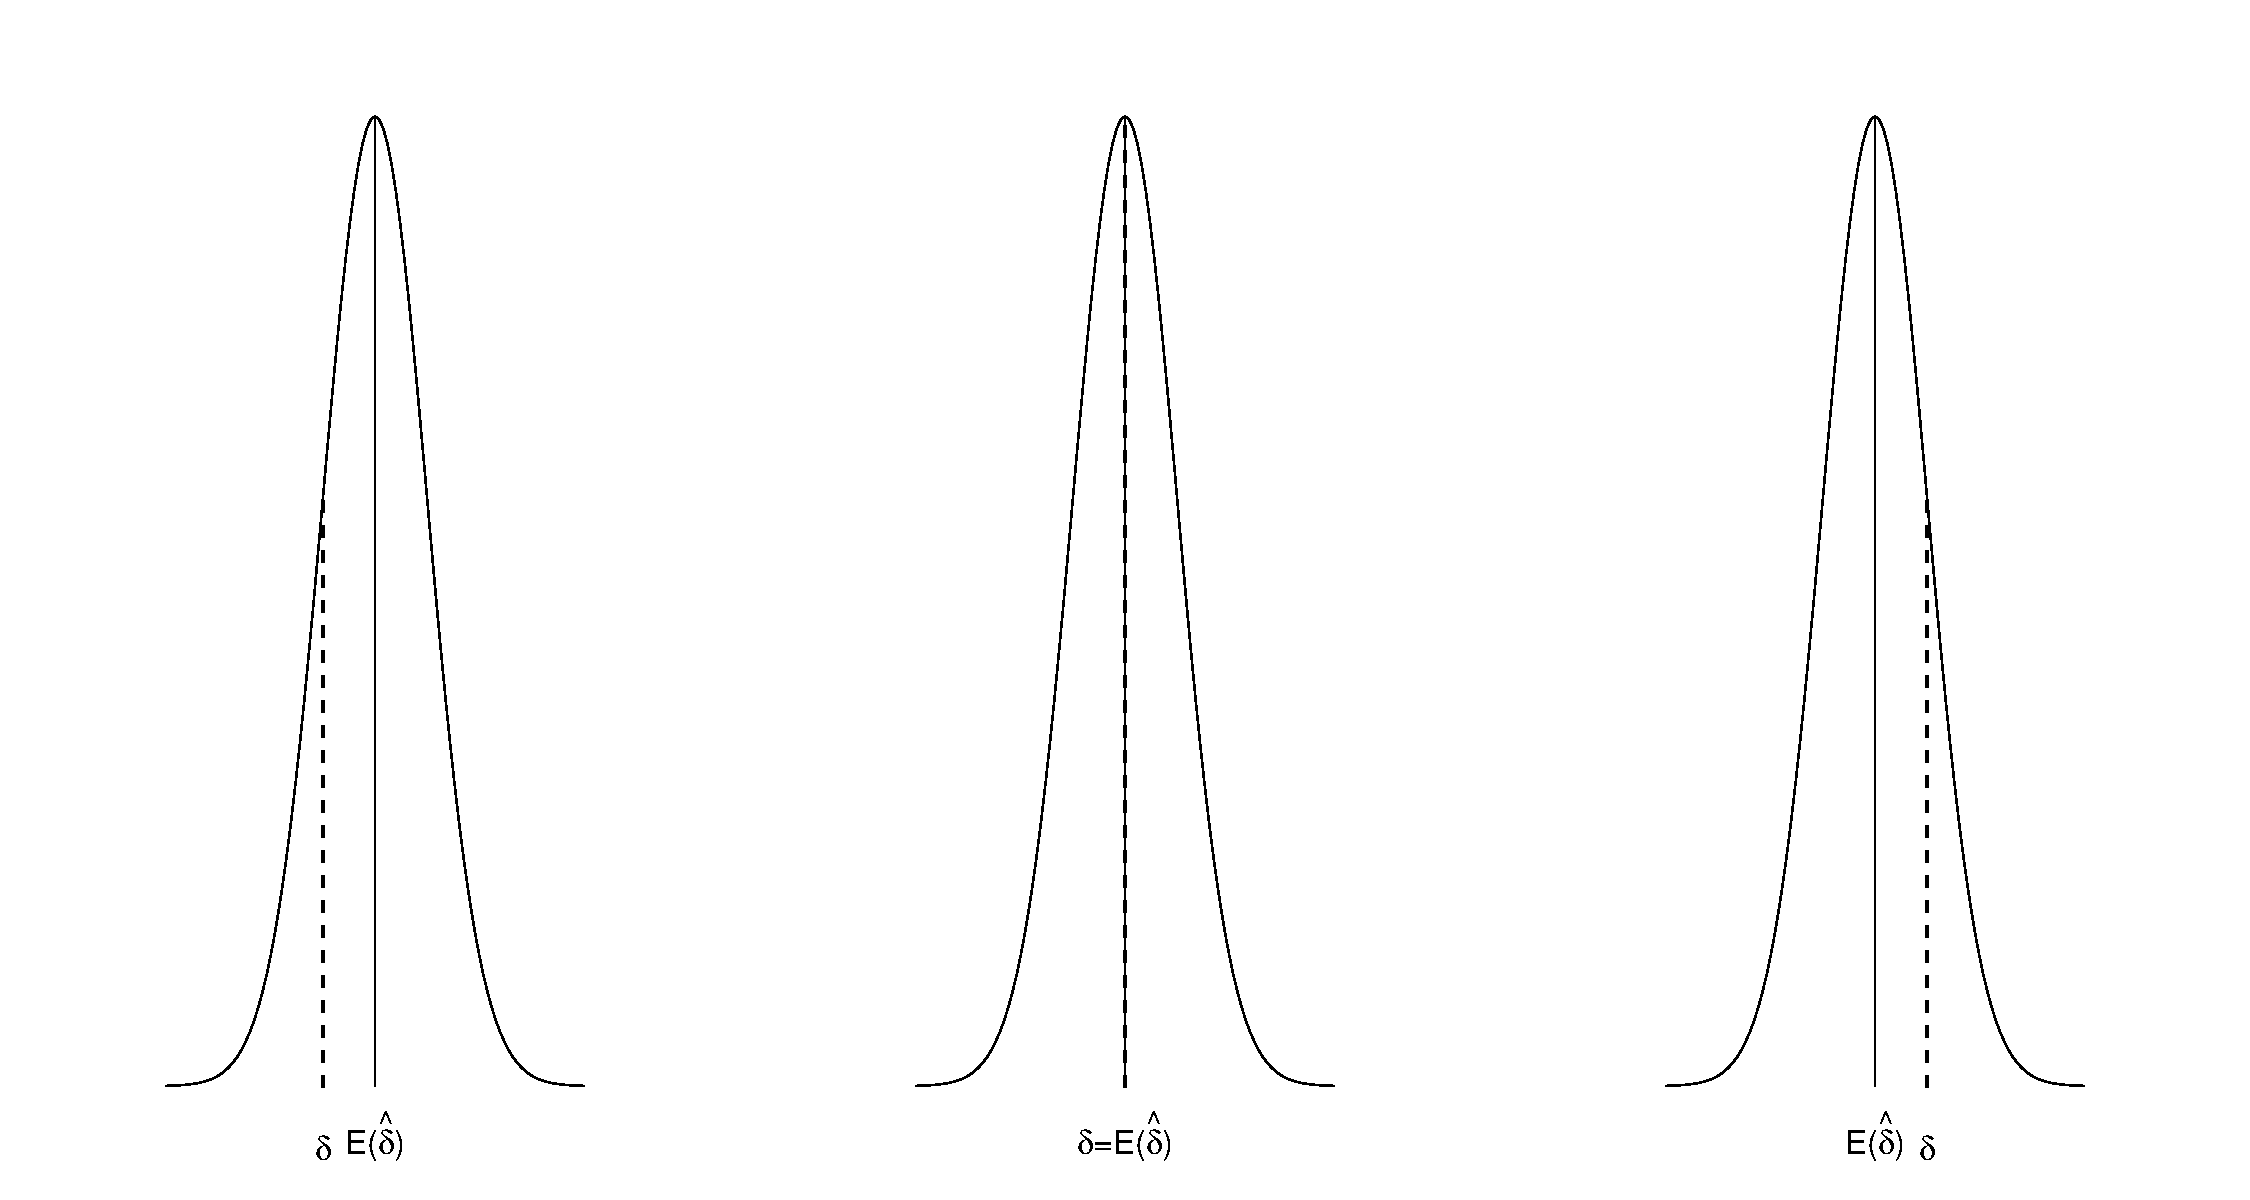
\includegraphics[width=400px]{ES_files/figure-latex/BIAS-1} \caption{Sampling distribution for a positively biased (left), an unbiased (center) and a negatively biased estimator (right)}\label{fig:BIAS}
\end{figure}

As we can see in Tables 1 and 2 the bias is directly related to the population effect size. The larger the population effect size, the larger the bias. As we shall see in the sequel, each effect size estimator actually estimates a different expression of the population effect size. It is therefore necessary to examine the \emph{relative bias}, defined as the ratio between the bias and the population effect size :
\begin{equation} 
\delta_{relative \; bias}=\frac{E(\hat{\delta})-\delta}{\delta}.
\label{eqn:RELBIAS}
\end{equation}
While the bias informs us about the quality of estimates on average, in particular their capacity of lying close to the true value, it says nothing about individual estimates. Imagine a situation where the distribution of estimates is centered around the real parameter but with such a large variance that some point estimates are very far from the center. This would be problematic, since any single estimate might be very far from the true population value. Therefore it is not only essential for an estimator to be unbiased, but it is also desirable that the variability of its sampling distribution is small. Ideally, all sample estimates are close to the true population parameter. Among two unbiased estimators \(\hat{\delta_1}\) and \(\hat{\delta_2}\), we therefore say that \(\hat{\delta_1}\) is \emph{more efficient} than \(\hat{\delta_2}\) if
\begin{equation} 
Var(\hat{\delta}_1) \leq Var(\hat{\delta}_2)
\label{eqn:EFFICIENCY}
\end{equation}
where \(Var(\hat{\delta})\) is the variance of the sampling distribution of the estimator \(\hat{\delta}\). This variance inequality of course only makes sense if two estimators \(\hat{\delta}_1\) and \(\hat{\delta}_2\) estimate the same population quantity, which is not the case here as explained before (each effect size estimator corresponds to a distinct population effect size expression). Therefore, we rather have to consider the \emph{relative variance}, defined as the ratio between the variance of an estimator and the square of the corresponding population effect size \(\delta\) :
\begin{equation} 
relative \; var(\hat{\delta})=\frac{Var(\hat{\delta})}{\delta^2}.
\label{eqn:RELVAR}
\end{equation}
Note that both unbiasedness and efficiency are very important when choosing an estimator. In some situations, it might be better to have a slightly biased estimator with low variance, (so that each estimate remains relatively close to the true parameter and one might be able to apply bias correction techniques) rather than an unbiased estimator with a large variance (Raviv, 2014).

Finally, the last property of a good point estimator is \emph{consistency}. Consistency means that the bigger the sample size, the closer the estimate is to the population parameter. In other words, the estimates \emph{converge} to the true population parameter.

\hypertarget{different-measures-of-effect-sizes}{%
\section{Different measures of effect sizes}\label{different-measures-of-effect-sizes}}

The \emph{d}-family effect sizes are commonly used for mean differences between groups or conditions. In all generality, the population effect size is defined as
\begin{equation} 
\delta = \frac{\mu_{1}-\mu_{2}}{\sigma} 
\label{eqn:Cohendelta}
\end{equation}
where \(\mu_1\) and \(\mu_2\) respectively stand for the population means of population 1 and 2, and \(\sigma\) represents the ``variability'' of the combined observations from both population. Typically one assumes that both populations are independent and normally distributed (the normality assumption however is often a too strong limitation; Delacre et al., 2017). In some situations it is moreover assumed that the variances of both populations are equal, in which case \(\sigma\) stands for the common standard deviation. There exist different estimators of the effect size measure in expression \ref{eqn:Cohendelta}. For all, the mean difference is estimated by the difference \(\bar{X}_1-\bar{X}_2\) of both sample means. When the equality of variances assumption is made, \(\sigma\) is estimated by pooling both sample standard deviations (\(S_1\) and \(S_2\)). When the equality of variances assumption cannot be made, the pooled standard deviation is a possible but not recommendable choice as we explain later on, and alternatives are available. In what follows, we shall present various effect size measures. For each effect size, we will provide information about their theoretical bias, variance and consistency. Simulation-based results will be discussed in the section ``Monte Carlo Simulations : assessing the bias, efficiency and consistency of 5 estimators'' below.

\hypertarget{cohens-bmd-and-hedges-bmg}{%
\subsection{\texorpdfstring{Cohen's \(\bm{d}\) and Hedges' \(\bm{g}\)}{Cohen's \textbackslash bm\{d\} and Hedges' \textbackslash bm\{g\}}}\label{cohens-bmd-and-hedges-bmg}}

When we have good reasons to assume equality of variances between groups then the most common effect size is Cohen's \(d\), where the sample mean difference is divided by a pooled error term (Cohen, 1965) :
\begin{equation*} 
Cohen's \; d = \frac{\bar{X}_1-\bar{X}_2}{\sqrt{\frac{(n_1-1) \times S_1^2+(n_2-1) \times S_2^2}{n_1+n_2-2}}}
\label{eqn:Cohends}
\end{equation*}
where \(S_j\) is the standard deviation, and \(n_j\) the sample size of the \(j^{th}\) sample (\(j=1,2\)). The reasoning behind this measure is to make use of the fact that both samples share the same population variance (Keselman et al., 2008), which means a more accurate estimation of the population variance can be achieved by pooling both estimates of this parameter (i.e.~\(S_1\) and \(S_2\)). Since the larger the sample size, the more accurate the estimate, we give more weight to the estimate based on the larger sample size. Cohen's \(d\) is directly related to Student's \emph{t}-statistic : \color{white} Keselman, Algina, Lix, Wilcox, and Deering (2008) \color{black}
\begin{equation} 
t_{Student}=\frac{Cohen's \; d}{\sqrt{\frac{1}{n_1}+\frac{1}{n_2}}}\leftrightarrow Cohen's \; d =  t_{Student} \times \sqrt{\frac{1}{n_1}+\frac{1}{n_2}}
\label{eqn:Cohenvsstudent}
\end{equation}
Under the assumption of normality and equal variances between groups, Student's \emph{t}-statistic follows a \emph{t}-distribution with known degrees of freedom
\begin{equation} 
df_{Student} = n_1+n_2-2
\label{eqn:studentdf}
\end{equation}
and noncentrality parameter\footnote{Under the null hypothesis of no differences between sample means, Student's $t$-statistic will follow a central $t$-distribution with $n_1+n_2-2$ degrees of freedom. However, when the null hypothesis is false, the distribution of this quantity will not be centered, and a noncentral $t$-distribution will arise.}
\[ncp_{Student} = \frac{\delta_{Cohen}}{\sqrt{\frac{1}{n_1}+\frac{1}{n_2}}}\]
where \(\delta_{Cohen}= \frac{\mu_1-\mu_2}{\sigma_{pooled}}\), \(\sigma_{pooled}= \sqrt{\frac{(n_1-1) \times \sigma^2_1+(n_2-1) \times \sigma^2_2}{n_1+n_2-2}}\) and \(\sigma_j\) is the standard deviation of the \(j^{th}\) population \((j=1,2)\). We attract the reader's attention to the act that \(\delta_{Cohen}\) is the expression of the effect size that the Cohen's \(d\) is estimating. The relationship described in equation \ref{eqn:Cohenvsstudent} and the theoretical distribution of Student's \emph{t}-statistic allow us to determine the sampling distribution of Cohen's \(d\), and therefore, its expectation and variance when the assumptions of normality and equal variances are met. All these equations are provided in Table 1. For interested readers, Supplemental Material 1 provides a detailed examination of the theoretical bias and variance of Cohen's \(d\) based on Table 1, as well as the bias and variance of all other estimators described later, based on Tables 2 and 3, with the goal to determine which parameters influence the bias and variance of different estimators.

While Cohen's \(d\) is a consistent estimator, its bias and variance are substantial with small sample sizes, even under the assumptions of normality and equal variances (Lakens, 2013). In order to compensate for Cohen's \(d\) bias with small sample sizes, Hedges and Olkin (1985) defined a bias-corrected version : \color{white} Hedges and Olkin (1985) \color{black}
\begin{equation*} 
Hedges' \; g = Cohen's \; d \times \frac{\Gamma(\frac{df_{Student}}{2})}{\sqrt{\frac{df_{Student}}{2}} \times \Gamma(\frac{df_{Student}-1}{2})}
\label{eqn:Hedgesgs}
\end{equation*}
where \(df_{Student}\) has been defined in equation \ref{eqn:studentdf} and \(\Gamma()\) is the gamma function (for integers, \(\Gamma(x)\) is the factorial of \(x\) minus \(1\) : \(\Gamma(x)=(x-1)!\); Goulet-Pelletier \(\&\) Cousineau, 2018). This equation can be approximated as follows : \color{white} Goulet-Pelletier and Cousineau (2018) \color{black}
\begin{equation*} 
Hedges' \; g = Cohen's \; d \times \left( 1- \frac{3}{4N -9} \right)
\label{eqn:Hedgesgsapprox}
\end{equation*}
where \(N\) is the total sample size. Hedges' \(g\) is theoretically unbiased when the assumptions of normality and equal variances are met (see Table 1). Moreover, while the variance of both Cohen's \(d\) and Hedges' \(g\) depend on the same parameters (i.e.~the total sample size (\(N\)) and the sample sizes ratio \(\left(\frac{n_2}{n_1}\right)\)), Hedges' \(g\) is less variable, especially with small sample sizes.\footnote{In Table 1, one can see that the variance of Hedges' $g$ equals the variance of Cohen's $d$, multiplied by $\left[\frac{\Gamma(\frac{df}{2})}{\sqrt{\frac{df}{2}} \times \Gamma(\frac{df-1}{2})} \right] ^2$. This term is always less than 1 and tends to 1 when the sample sizes tend to infinity ($.52 \le \left[\frac{\Gamma(\frac{df}{2})}{\sqrt{\frac{df}{2}} \times \Gamma(\frac{df-1}{2})} \right] ^2 < 1$ for $3 \le df < \infty$). As a consequence, the larger the total sample size, the smaller the difference between the variance of Cohen's $d$ and Hedges' $g$.} \color{white} Cumming (2013) Grissom and Kim (2005) Kelley (2005)\color{black}

While the pooled error term is the best choice when variances are equal between groups (Grissom \& Kim, 2001), it may not be well advised for use with data that violate this assumption (Cumming, 2013; Grissom \& Kim, 2001; Grissom \& Kim, 2005; Kelley, 2005; Shieh, 2013). When variances are unequal between groups, the expression in equation \ref{eqn:Cohendelta} is no longer valid because both groups do not share a common population variance. If we pool the estimates of two unequal population variances, the estimator of effect size will be smaller as it should be in case of positive pairing (i.e.~the group with the larger sample size is extracted from the population with the larger variance) and larger as it should be in case of negative pairing (i.e.~the group with the larger sample size is extracted from the population with the smaller variance).

\newpage
\begin{landscape}

\begin{longtable}[]{@{}
  >{\raggedright\arraybackslash}p{(\columnwidth - 6\tabcolsep) * \real{0.13}}
  >{\centering\arraybackslash}p{(\columnwidth - 6\tabcolsep) * \real{0.12}}
  >{\centering\arraybackslash}p{(\columnwidth - 6\tabcolsep) * \real{0.27}}
  >{\centering\arraybackslash}p{(\columnwidth - 6\tabcolsep) * \real{0.48}}@{}}
\caption{Expectation, bias and variance of Cohen's \(d\) and Hedges' \(g\) under the assumptions that independent residuals are normally distributed with equal variances across groups.}\tabularnewline
\toprule
\begin{minipage}[b]{\linewidth}\raggedright
\end{minipage} & \begin{minipage}[b]{\linewidth}\centering
df
\end{minipage} & \begin{minipage}[b]{\linewidth}\centering
Expectation
\end{minipage} & \begin{minipage}[b]{\linewidth}\centering
Variance
\end{minipage} \\
\midrule
\endfirsthead
\toprule
\begin{minipage}[b]{\linewidth}\raggedright
\end{minipage} & \begin{minipage}[b]{\linewidth}\centering
df
\end{minipage} & \begin{minipage}[b]{\linewidth}\centering
Expectation
\end{minipage} & \begin{minipage}[b]{\linewidth}\centering
Variance
\end{minipage} \\
\midrule
\endhead
Cohen's \(d\) & \(N-2\) & \(\delta_{Cohen} \times c_f\) & \(\frac{N\times df}{n_1n_2 \times (df-2)} + \delta^2_{Cohen} \left[ \frac{df}{df-2} - c_f^2\right]\) \\
& & & \\
& & \(\approx \frac{\delta_{Cohen}}{\left(1-\frac{3}{4N-9}\right)}\) & \(\approx \frac{N\times df}{n_1n_2 \times (df-2)} + \delta^2_{Cohen} \left[ \frac{df}{df-2} - \left( \frac{1}{1-\frac{3}{4N-9} }\right)^2\right]\) \\
& & & \\
& & & \\
Hedges' \(g\) & \(N-2\) & \(\delta_{Cohen}\) & \(Var(Cohen's \; d_s) \times \left[ \frac{\Gamma(\frac{df}{2})}{\sqrt{\frac{df}{2}} \times \Gamma(\frac{df-1}{2})} \right]^2\) \\
& & & \\
& & & \(\approx Var(Cohen's \; d_s) \times \left[1-\frac{3}{4N-9}\right]^2\) \\
& & & \\
\bottomrule
\end{longtable}

\emph{Note}. \(\delta_{Cohen}= \frac{\mu_1-\mu_2}{\sigma_{pooled}}\) and \(c_f=\frac{\sqrt{\frac{df}{2}} \times \Gamma\left( \frac{df-1}{2}\right)}{\Gamma\left( \frac{df}{2}\right)}\); Cohen's \(d\) is a biased estimator, because its expectation differs from the population effect size. Moreover, the larger the population estimator (\(\delta_{Cohen}\)), the larger the bias. Indeed, the bias is the difference between the expectation and \(\delta_{Cohen}\): \(\delta_{bias} = \delta_{Cohen} \times (c_f-1)\). On the other hand, Hedges' \(g\) is an unbiased estimator, because its expectation equals \(\delta_{Cohen}\); equations in this table require \(df \ge 3\) (i.e.~\(N \ge 5\)).

\end{landscape}

\hypertarget{three-popular-alternatives-from-the-literature}{%
\subsection{Three popular alternatives from the literature}\label{three-popular-alternatives-from-the-literature}}

In his review, Shieh (2013) mentions three options available in the literature to deal with the case of unequal variances : (A) the Glass' \(d\), (B) the Shieh's \(d\) and (C) the Cohen's \(d^*\).

\hypertarget{glass-bmd}{%
\subsubsection{\texorpdfstring{Glass' \(\bm{d}\)}{Glass' \textbackslash bm\{d\}}}\label{glass-bmd}}

When comparing one control group with one experimental group, Glass et al.~(1981) recommend using the standard deviation of the control group as standardizer. This yields \color{white} Glass, McGaw, and Smith (1981) \color{black}
\begin{equation*} 
Glass' \; d = \frac{\bar{X}_{e} - \bar{X}_{c}}{S_{c}}
\label{eqn:Glassds}
\end{equation*}
where \(\bar{X}_{e}\) and \(\bar{X}_{c}\) are the sample means of the experimental and control groups, and \(S_{c}\) is the sample \(SD\) of the control group. One argument in favour of using \(S_c\) as standardizer is the fact that it is not affected by the experimental treatment. When it is easy to identify which group is the ``control'' one, it is therefore convenient to compare the effect size estimation of different designs studying the same effect (Cumming, 2013). However, defining this group is not always obvious (Coe, 2002). This could induce large ambiguity because depending on the chosen \(SD\) as standardizer, measures could be substantially different (Shieh, 2013). As we shall see later through our simulations, this estimator also does not present good inferential properties. The distribution of Glass' \(d\) is defined as in Algina et al.~(2006) : \color{white} Algina, Keselman, and Penfield (2006) \color{black}
\begin{equation} 
Glass' \; d \sim \sqrt{\frac{1}{n_{c}}+\frac{\sigma_{e}^2}{n_{e} \times \sigma^2_{c}}} \times t_{df,ncp}
\label{eqn:glassvst}
\end{equation}
where \(n_c\) and \(n_e\) are the sample sizes of the control and experimental groups, \(\sigma^2_c\) and \(\sigma^2_e\) are the population variance of the control and experimental groups and and \(df\) and \(ncp\) are defined as follows :
\begin{equation} 
df = n_{c}-1
\label{eqn:glassdf}
\end{equation}
\begin{equation*} 
ncp = \frac{\delta_{Glass}}{\sqrt{\frac{1}{n_{c}} + \frac{\sigma_{e}^2}{n_{e} \times \sigma^2_{c}}}}
\label{eqn:glassncp}
\end{equation*}
where \(\delta_{Glass} = \frac{\mu_{c}-\mu_{e}}{\sigma_{c}}\) and \(\mu_c\) and \(\mu_e\) are respectively the mean of the populations control and experimental groups are extracted from. Note that here the population effect size \(\delta_{Glass}\) is also based on the standard deviation \(\sigma_c\) of the control group. Thanks to equation \ref{eqn:glassvst}, we can compute the theoretical expectation and variance of Glass's \(d\) when the assumption of normality is met (see Table 2), and therefore determine which factors influence bias and variance, and how they do so (see Supplemental Material 1).

\newpage
\begin{landscape}

\begin{longtable}[]{@{}
  >{\raggedright\arraybackslash}p{(\columnwidth - 6\tabcolsep) * \real{0.11}}
  >{\centering\arraybackslash}p{(\columnwidth - 6\tabcolsep) * \real{0.20}}
  >{\centering\arraybackslash}p{(\columnwidth - 6\tabcolsep) * \real{0.18}}
  >{\centering\arraybackslash}p{(\columnwidth - 6\tabcolsep) * \real{0.51}}@{}}
\caption{Expectation, bias and variance of Glass' \(d\) and Cohen's \(d^*\) and Shieh's \(d\) under the assumption that independent residuals are normally distributed.}\tabularnewline
\toprule
\begin{minipage}[b]{\linewidth}\raggedright
\end{minipage} & \begin{minipage}[b]{\linewidth}\centering
df
\end{minipage} & \begin{minipage}[b]{\linewidth}\centering
Expectation
\end{minipage} & \begin{minipage}[b]{\linewidth}\centering
Variance
\end{minipage} \\
\midrule
\endfirsthead
\toprule
\begin{minipage}[b]{\linewidth}\raggedright
\end{minipage} & \begin{minipage}[b]{\linewidth}\centering
df
\end{minipage} & \begin{minipage}[b]{\linewidth}\centering
Expectation
\end{minipage} & \begin{minipage}[b]{\linewidth}\centering
Variance
\end{minipage} \\
\midrule
\endhead
Glass' \(d\) & \(n_c-1\) & ~\(\delta_{Glass} \times c_f\) & \(\frac{df}{df-2} \times \left( \frac{1}{n_c} + \frac{\sigma^2_e}{n_e\sigma^2_c}\right) + \delta^2_{Glass} \left( \frac{df}{df-2} - c_f^2 \right)\) \\
& & & \\
Cohen's \(d^*\) & \(\frac{(n_1-1)(n_2-1)(\sigma^2_1+\sigma^2_2)^2}{(n_2-1)\sigma^4_1+(n_1-1)\sigma^4_2}\) & \(\delta^*_{Cohen} \times c_f\) & \(\frac{df}{df-2} \times \frac{2\left( \frac{\sigma^2_1}{n_1} + \frac{\sigma^2_2}{n_2} \right)}{\sigma^2_1+\sigma^2_2} + (\delta^*_{Cohen})^2 \left( \frac{df}{df-2} - c_f^2 \right)\) \\
& & & \\
& & \(\approx \delta^*_{Cohen} \times \frac{4df-1}{4(df-1)}\) & \(\approx \frac{df}{df-2} \times \frac{2\left( \frac{\sigma^2_1}{n_1} + \frac{\sigma^2_2}{n_2} \right)}{\sigma^2_1+\sigma^2_2} + (\delta^*_{Cohen})^2 \left[ \frac{df}{df-2} - \left( \frac{4 \;df-1}{4(df-1)}\right)^2 \right]\) \\
& & & \\
Shieh's \(d\) & \(\frac{\left(\frac{\sigma^2_1}{n_1}+\frac{\sigma^2_2}{n_2} \right)^2}{\frac{(\sigma^2_1/n_1)^2}{n_1-1}+\frac{(\sigma^2_2/n_2)^2}{n_2-1}}\) & \(\delta_{Shieh} \times c_f\) & \(\frac{df}{(df-2)N} + \delta^2_{Shieh} \left( \frac{df}{df-2} - c_f^2 \right)\) \\
& & & \\
\bottomrule
\end{longtable}

\emph{Note}. \(c_f=\frac{\sqrt{\frac{df}{2}} \times \Gamma\left( \frac{df-1}{2}\right)}{\Gamma\left( \frac{df}{2}\right)}\); \(\delta_{Glass}=\frac{\mu_c-\mu_e}{\sigma_c}\), \(\delta_{Shieh}=\frac{\mu_1-\mu_2}{\sqrt{\frac{\sigma^2_1}{n_1/N}+\frac{\sigma^2_2}{n_2/N}}}\) and \(\delta^*_{Cohen}=\frac{\mu_1-\mu_2}{\sqrt{\frac{\sigma^2_1+\sigma^2_2}{2}}}\); all estimators are biased estimators, because their expectations differ from the population effect size \(\delta\). Moreover, the larger the population estimator (\(\delta\)), the larger the bias. Indeed, the bias is the difference between the expectation and \(\delta\): \(\delta_{bias} = \delta \times (c_f-1)\); equations in this table require \(df \ge 3\) and at least 2 subjects per group.

\end{landscape}
\newpage

\hypertarget{shiehs-bmd}{%
\subsubsection{\texorpdfstring{Shieh's \(\bm{d}\)}{Shieh's \textbackslash bm\{d\}}}\label{shiehs-bmd}}

Kulinskaya and Staudte (2007) were the first to recommend the use of a standardizer that takes the sample sizes allocation ratios into account, in addition to the variance of both samples. Shieh (2013), following Kulinskaya and Staudte, proposed a modification of the exact \emph{SD} of the sample mean difference : \color{white} Kulinskaya and Staudte (2007) \color{black}
\begin{equation*} 
Shieh's \; d = \frac{\bar{X}_1 - \bar{X}_2}{\sqrt{S_1^2/q_1+S_2^2/q_2}}; \;\;\; q_j=\frac{n_j}{N} (j=1,2)
\label{eqn:Shiehds}
\end{equation*}
where \(N = n_1+n_2\). Shieh's \(d\) is directly related with Welch's \emph{t}-statistic :
\begin{equation} 
Shieh's \; d=\frac{t_{Welch}}{\sqrt{N}}\leftrightarrow t_{welch} = Shieh's \; d \times \sqrt{N}.
\label{eqn:shiehvswelch}
\end{equation}
The exact distribution of Welch's \emph{t}-statistic is more complicated than the exact distribution of Student's \emph{t}-statistic, but it can be approximated, under the assumption of normality, by a \emph{t}-distribution with degrees of freedom and noncentrality parameters (Welch, 1938)
\begin{equation} 
df_{Welch} = \frac{\left(\frac{\sigma^2_1}{n_1}+\frac{\sigma^2_2}{n_2} \right)^2}{\frac{(\sigma^2_1/n_1)^2}{n_1-1}+\frac{(\sigma^2_2/n_2)^2}{n_2-1}}
\label{eqn:welchdf}
\end{equation}
\begin{equation*} 
ncp_{Welch} = \delta_{Shieh} \times \sqrt{N} = \frac{\mu_1-\mu_2}{\sqrt{\frac{\sigma_1^2}{n1}+\frac{\sigma_2^2}{n_2}}}
\label{eqn:welchncp}
\end{equation*}
where \(\delta_{Shieh}=\frac{\mu_1-\mu_2}{\sqrt{\frac{\sigma_1^2}{n_1/N}+\frac{\sigma_2^2}{n_2/N}}}\) is the population effect size measure estimated by Shieh's \(d\). The relationship described in equation \ref{eqn:shiehvswelch} and the theoretical distribution of Welch's \emph{t}-statistic allow us to approximate the sampling distribution of Shieh's \(d\). Based on the sampling distribution of Shieh's \(d\), we can estimate its theoretical expectation and variance under the assumption of normality (see Table 2), and thereby determine which factors influence bias and variance, and how they do so (see Supplemental Material 1).

As demonstrated in Appendices 1 and 2, when population variances and sample sizes are equal across groups, the biases and variances of Cohen's \(d\) and Shieh's \(d\) are identical except for multiplication by a constant. The same is true for the population effect size expressions \(\delta_{Cohen}\) and \(\delta_{Shieh}\) :\\
\begin{equation} 
\delta_{Cohen} = 2 \times \delta_{Shieh} \quad (\mbox{considering} \; \sigma_1 = \sigma_2 \; \mbox{and} \; n_1 = n_2)
\label{eqn:CohenShieh}
\end{equation}
\begin{equation} 
Bias_{Cohen's \; d} = 2 \times Bias_{Shieh's \; d} \quad (\mbox{considering} \; \sigma_1 = \sigma_2 \; \mbox{and} \; n_1 = n_2)
\label{eqn:biasCohenshieh}
\end{equation}
\begin{equation} 
Var_{Cohen's \; d} = 4 \times Var_{Shieh's \; d} \quad (\mbox{considering}\; \sigma_1 = \sigma_2 \; \mbox{and} \; n_1 = n_2)
\label{eqn:varCohenshieh}
\end{equation}
We can deduce from equations \ref{eqn:CohenShieh}, \ref{eqn:biasCohenshieh} and \ref{eqn:varCohenshieh} that relative to their respective population effect size, Cohen's \(d\) and Shieh's \(d\) are equally accurate. In other words, their relative bias and variance are identical.

When sample sizes are not equal, according to the statistical properties of Welch's statistic under heteroscedasticity, Shieh's \(d\) accounts for the allocation ratio of sample sizes to each condition. The lack of generality caused by taking this specificity of the design into account has led Cumming (2013) to question its usefulness in terms of interpretability : when the mean difference (\(\bar{X_1}-\bar{X_2}\)), \(S_1\), and \(S_2\) remain constant, Shieh's \(d\) will vary as a function of the sample sizes allocation ratio (unlike Cohen's \(d^*\) that we will define below). At the population level, \(\delta_{Shieh}\) also depends on the sample sizes allocation ratio, as illustrated in the following shiny application : \url{https://effectsize.shinyapps.io/ShiehvsCohen/}.

\hypertarget{cohens-bmd}{%
\subsubsection{\texorpdfstring{Cohen's \(\bm{d^*}\)}{Cohen's \textbackslash bm\{d\^{}*\}}}\label{cohens-bmd}}

An effect size estimator based on the sample mean difference divided by the square root of the non pooled average of both variance estimates was suggested by Welch (1938). Here, we indicate the difference between Cohen's \(d\) (based on the pooled standard deviations) and Cohen's \(d^*\) with an asterisk. This yields :
\begin{equation*} 
Cohen's \; d^* = \frac{\bar{X}_{1} - \bar{X}_{2}}{ \sqrt{\frac{\left(S^2_{1}+S^2_{2} \right)}{2}}}
\label{eqn:Cohenprimeds}
\end{equation*}
where \(\bar{X}_{j}\) is the mean and \(S_j\) is the standard deviation of the \(j^{th}\) sample (j = 1,2). We know the distribution of Cohen's \(d^*\) (Huynh, 1989) :
\begin{equation} 
Cohen's \; d^* \sim  \sqrt{\frac{2(n_2\times\sigma^2_1+n_1\times\sigma^2_2)}{n_1n_2(\sigma^2_1+\sigma^2_2)}} \times t_{df^*,ncp^*}
\label{eqn:Cohendprimedist}
\end{equation}
where \(df^*\) and \(ncp^*\) are defined as follows :
\begin{equation} 
df^* = \frac{(n_1-1)(n_2-1)(\sigma^2_1+\sigma^2_2)^2}{(n_2-1)\sigma^4_1+(n_1-1)\sigma^4_2}
\label{eqn:Cohendprimedf}
\end{equation}
\begin{equation*} 
ncp^*=\delta^*_{Cohen} \times \sqrt{\frac{n_1n_2(\sigma^2_1+\sigma^2_2)}{2(n_2\sigma^2_1+n_1\sigma^2_2)}}=\frac{\mu_1-\mu_2}{\sqrt{\frac{\sigma_1^2}{n_1}+\frac{\sigma^2_2}{n_2}}}
\label{eqn:Cohendprimevst}
\end{equation*}
where \(\delta^*_{Cohen}=\frac{\mu_1-\mu_2}{\sqrt{\frac{\sigma^2_1+\sigma^2_2}{2}}}\) is the corresponding population effect size. Using equation \ref{eqn:Cohendprimedist} we can compute its theoretical expectation and variance when the assumption of normality is met (see Table 2), and therefore determine which factors influence bias and variance, and how they do so (see Supplemental Material 1). This estimator has been widely criticized, because it results in a variance term of an artificial population (i.e.~since the variance term does not estimate the variance of one or the other group, the composite variance is an estimation of the variance of an artificial population; Grissom \(\&\) Kim, 2001). However, the same criticism would then apply to the celebrated Cohen's \(d\) because the pooled variance also corresponds to the variance of an artificial population, unless when variances are equal. But for equal variances the variance term of Cohen's \(d^*\) also yields \(\sigma^2\), which is perfectly interpretable. Moreover, we will show throughout the simulation section that this estimator exhibits very good inferential properties. Moreover, it has a constant value across sample sizes ratios, as shown in the Shiny App at \url{https://effectsize.shinyapps.io/ShiehvsCohen/}.

\hypertarget{glass-bmg-shiehs-bmg-and-hedges-bmg}{%
\subsubsection{\texorpdfstring{Glass' \(\bm{g}\), Shieh's \(\bm{g}\) and Hedges' \(\bm{g^*}\)}{Glass' \textbackslash bm\{g\}, Shieh's \textbackslash bm\{g\} and Hedges' \textbackslash bm\{g\^{}*\}}}\label{glass-bmg-shiehs-bmg-and-hedges-bmg}}

As for Cohen's \(d\), a Hedges' correction can be applied in order to compensate for the bias of Glass' \(d\), Shieh's \(d\) and Cohen's \(d^*\) with small sample sizes (see Table 2). This correction has the following general form :
\begin{equation*} 
g = d \times \frac{\Gamma(\frac{\nu}{2})}{\sqrt{\frac{\nu}{2}} \times \Gamma(\frac{\nu-1}{2})}
\end{equation*}
where the distinct values of \(\nu\) are provided in equation \ref{eqn:glassdf} for Glass' \(g\), in equation \ref{eqn:welchdf} for Shieh's \(g\) and in equation \ref{eqn:Cohendprimedf} for Hedges' \(g^*\). The three corrected estimators are theoretically unbiased when the assumption of normality is met. Their variance is a function of the same parameters as their biased equivalent. However, due to the correction they have a smaller variance, especially with small sample sizes, as shown in Table 3. In summary :

\begin{itemize}
\tightlist
\item
  The variances of Hedges' \(g^*\) and Shieh's \(g\) depend on the total sample size (\(N\)), their respective population effect size (\(\delta\)), and the interaction between the sample sizes ratio and the \(SD\)-ratio \(\left(\frac{n_2}{n_1}\times\frac{\sigma_2}{\sigma_1} \right)\).\\
\item
  The variance of Glass' \(g\) also depends on \(N\), \(\delta\) and \(\frac{n_c}{n_e}\times\frac{\sigma_c}{\sigma_e}\). In addition, there is also a main effect of the \(SD\)-ratio \(\left(\frac{\sigma_c}{\sigma_e} \right)\) on its variance.
\end{itemize}

How these parameters influence the variance of the estimators will be summarized and illustrated in Monte Carlo simulations below.

\newpage
\begin{landscape}

\begin{longtable}[]{@{}
  >{\raggedright\arraybackslash}p{(\columnwidth - 6\tabcolsep) * \real{0.11}}
  >{\centering\arraybackslash}p{(\columnwidth - 6\tabcolsep) * \real{0.20}}
  >{\centering\arraybackslash}p{(\columnwidth - 6\tabcolsep) * \real{0.18}}
  >{\centering\arraybackslash}p{(\columnwidth - 6\tabcolsep) * \real{0.51}}@{}}
\caption{Expectation, bias and variance of Glass' \(g\), Hedges' \(g^*\) and Shieh's \(g\) under the assumption that independent residuals are normally distributed.}\tabularnewline
\toprule
\begin{minipage}[b]{\linewidth}\raggedright
\end{minipage} & \begin{minipage}[b]{\linewidth}\centering
df
\end{minipage} & \begin{minipage}[b]{\linewidth}\centering
Expectation
\end{minipage} & \begin{minipage}[b]{\linewidth}\centering
Variance
\end{minipage} \\
\midrule
\endfirsthead
\toprule
\begin{minipage}[b]{\linewidth}\raggedright
\end{minipage} & \begin{minipage}[b]{\linewidth}\centering
df
\end{minipage} & \begin{minipage}[b]{\linewidth}\centering
Expectation
\end{minipage} & \begin{minipage}[b]{\linewidth}\centering
Variance
\end{minipage} \\
\midrule
\endhead
Glass' \(g\) & \(n_c-1\) & ~\(\delta_{glass}\) & \(Var(Glass' \; d) \times \left( \frac{\Gamma\left(\frac{df}{2} \right)}{\sqrt{\frac{df}{2}} \times \Gamma \left( \frac{df-1}{2}\right)}\right)^2\) \\
& & & \\
Hedges' \(g^*\) & \(\frac{(n_1-1)(n_2-1)(\sigma^2_1+\sigma^2_2)^2}{(n_2-1)\sigma^4_1+(n_1-1)\sigma^4_2}\) & \(\delta^*_{Cohen}\) & \(Var(Cohen's \; d^*_s) \times \left( \frac{\Gamma\left(\frac{df}{2} \right)}{\sqrt{\frac{df}{2}} \times \Gamma \left( \frac{df-1}{2}\right)}\right)^2\) \\
& & & \\
Shieh's \(g\) & \(\approx \frac{\left(\frac{\sigma^2_1}{n_1}+\frac{\sigma^2_2}{n_2} \right)^2}{\frac{(\sigma^2_1/n_1)^2}{n_1-1}+\frac{(\sigma^2_2/n_2)^2}{n_2-1}}\) & \(\delta_{Shieh}\) & \(Var(Shieh's \; d) \times \left( \frac{\Gamma\left(\frac{df}{2} \right)}{\sqrt{\frac{df}{2}} \times \Gamma \left( \frac{df-1}{2}\right)}\right)^2\) \\
& & & \\
\bottomrule
\end{longtable}

\emph{Note}. \(c_f=\frac{\sqrt{\frac{df}{2}} \times \Gamma\left( \frac{df-1}{2}\right)}{\Gamma\left( \frac{df}{2}\right)}\); \(\delta_{Glass}=\frac{\mu_c-\mu_e}{\sigma_c}\), \(\delta_{Shieh}=\frac{\mu_1-\mu_2}{\sqrt{\frac{\sigma^2_1}{n_1/N}+\frac{\sigma^2_2}{n_2/N}}}\) and \(\delta^*_{Cohen}=\frac{\mu_1-\mu_2}{\sqrt{\frac{\sigma^2_1+\sigma^2_2}{2}}}\); all estimators are unbiased estimators, because their expectations equal the population effect size \(\delta\); equations in this table require \(df \ge 3\) and at least 2 subjects per group.

\end{landscape}
\newpage

\hypertarget{monte-carlo-simulations}{%
\subsection{Monte Carlo Simulations}\label{monte-carlo-simulations}}

\hypertarget{assessing-the-bias-efficiency-and-consistency-of-5-estimators}{%
\subsubsection{Assessing the bias, efficiency and consistency of 5 estimators}\label{assessing-the-bias-efficiency-and-consistency-of-5-estimators}}

\hypertarget{method}{%
\paragraph{Method}\label{method}}

We performed Monte Carlo simulations using R (version 3.5.0) to assess the bias, efficiency and consistency of Hedges' \(g\), Glass' \(g\) (using respectively the sample \(SD\) of the first or second group as a standardizer), Hedges' \(g^*\) and Shieh's \(g\).

A set of 100,000 datasets was generated for 1,008 scenarios as a function of different criteria. In 252 scenarios, samples were extracted from a normally distributed population (in order to ensure the reliability of our calculation method) and in 756 scenarios, samples were extracted from non normal population distributions. In order to assess the quality of estimators under realistic deviations from the normality assumption, we referred to the review of Cain et al.~(2017). Cain et al.~(2017) investigated 1,567 univariate distributions from 194 studies published by authors in Psychological Science (from January 2013 to June 2014) and the American Education Research Journal (from January 2010 to June 2014). For each distribution, they computed Fisher's skewness \color{white} Cain, Zhang, and Yuan (2017) \color{black}
\[G_{1}=\frac{\sqrt{n(n-1)}}{n-2} \frac{m_{3}}{\sqrt{(m_{2})^3}}\]
and kurtosis \[G_{2}=\frac{n-1}{(n-2)(n-3)}\times \left[(n+1)\left(\frac{m_{4}}{(m_{2})^2}-3\right)+6\right]\]
where \(n\) is the sample size and \(m_{2}\), \(m_{3}\) and \(m_{4}\) are respectively the second, third and fourth centered moments. They found values of kurtosis from \(G_2\) = -2.20 to 1,093.48. According to their suggestions, throughout our simulations, we kept constant the population kurtosis value at the 99th percentile of their distribution of kurtosis, i.e.~\(G_2=95.75\). Regarding skewness, we simulated population parameter values which correspond to the 1st and 99th percentile of their distribution of skewness, i.e.~respectively \(G_1\) = -2.08 and \(G_1\) = 6.32. We also simulated samples extracted from population where \(G_1\) = 0, in order to assess the main effect of high kurtosis on the quality of estimators. All possible combinations of population skewness and kurtosis and the number of scenarios for each combination are summarized in Table 4. To provide the reader with an intuition about the four distributions we consider, we have plotted them in Figure \ref{fig:DISTR}.

\begin{figure}
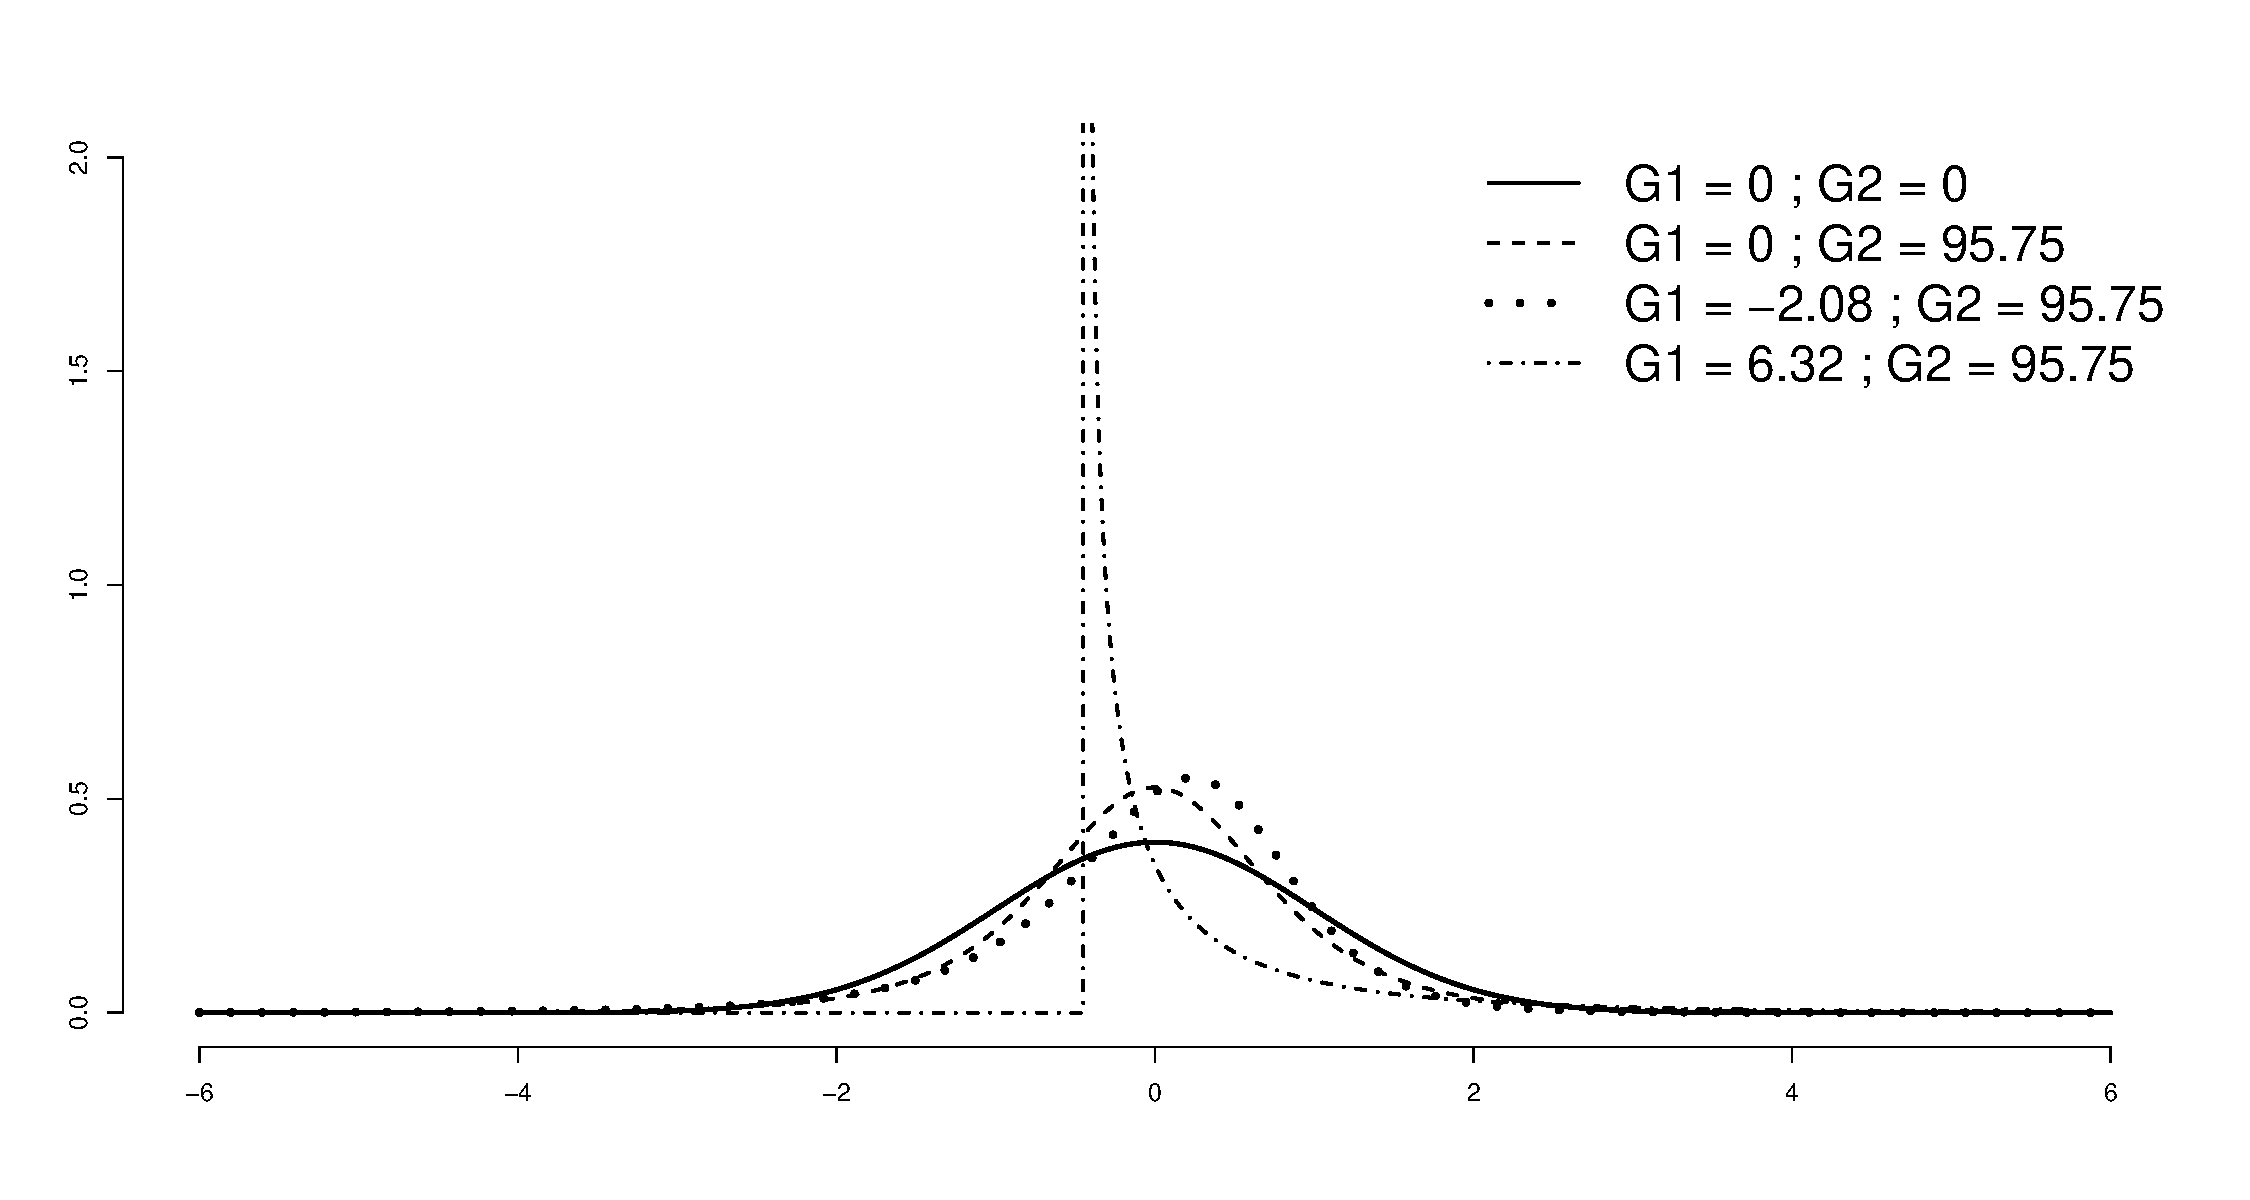
\includegraphics[width=400px]{ES_files/figure-latex/DISTR-1} \caption{Plots of the four distributions considered in our simulations, with $\mu=0$ and $\sigma=1$. The undotted curve is the normal distribution.}\label{fig:DISTR}
\end{figure}

\begin{longtable}[]{@{}ccccc@{}}
\caption{Number of combinations of skewness and kurtosis in our simulations.}\tabularnewline
\toprule
& & & \textbf{Kurtosis} & \\
\midrule
\endfirsthead
\toprule
& & & \textbf{Kurtosis} & \\
\midrule
\endhead
& & 0 & 95.75 & \textbf{TOTAL} \\
& & --------------- & -------------- & --------------- \\
& 0 & 252 & 252 & \textbf{504} \\
& & & & \\
\textbf{Skewness} & -2.08 & / & 252 & \textbf{252} \\
& & & & \\
& 6.32 & / & 252 & \textbf{252} \\
& & & & \\
& \textbf{TOTAL} & \textbf{252} & \textbf{756} & \textbf{1008} \\
\bottomrule
\end{longtable}

\emph{Note.} Fisher's skewness (G1) and kurtosis (G2) are presented in Table 4. The 252 combinations where both G1 and G2 equal 0 correspond to the normal case.

For the 4 resulting combinations of skewness and kurtosis (see Table 4), all other parameter values were chosen in order to illustrate the consequences of factors identified as playing a key role on the variance of unbiased estimators. We manipulated the population mean difference (\(\mu_1-\mu_2\)), the sample sizes (\(n_1\) and \(n_2\)), the sample size ratio (\emph{n}-ratio = \(\frac{n_2}{n_1}\)), the population \emph{SD}-ratio (i.e.~\(\frac{\sigma_2}{\sigma_1}\)), and the sample size and population variance pairing \(\left(\frac{n_2}{n_1}\times\frac{\sigma_2}{\sigma_1} \right)\). In our scenarios, \(\mu_2\) was always 0 and \(\mu_1\) varied from 1 to 4, in steps of 1 (so does \(\mu_1-\mu_2\)). Thus, we only consider a positive population effect size, which will result in positive bias of our estimators for reasons explained in Supplemental Material 1. \footnote{In the original plan, we had added 252 simulations in which $\mu_1$ and $\mu_2$ were both null. We decided not to present the results of these simulations in the main article, because the relative bias and the relative variance appeared to us to be very useful to fully understand the comparison of the estimators, and computing them is impossible when the real mean difference is zero. Indeed, for these specific configurations, both relative bias and relative variance would have infinite values due to the presence of the population effect size term in their denominator. However, these extra simulations were included in the simulation checks, in Supplemental Material 2. } Moreover, \(\sigma_1\) always equals 1, and \(\sigma_2\) equals .1, .25, .5, 1, 2, 4 or 10, and therefore, the \(SD\)-ratio were 10, 4, 2, 1, .5, .25 or .1. The simulations for which both \(\sigma_1\) and \(\sigma_2\) equal 1 are the particular case of homoscedasticity, or equal population variances across groups. The sample sizes of both groups (\(n_1\) and \(n_2\)) were 20, 50 or 100. When sample sizes of both groups are equal, the \emph{n}-ratio equals 1 (this is known as a balanced design). All possible combinations of \emph{n}-ratio and population \emph{SD}-ratio were simulated in order to distinguish scenarios where both sample sizes and population variances are unequal across groups (with positive pairing when the group with the largest sample size is extracted from the population with the largest \emph{SD}, and negative pairing when the group with the smallest sample size is extracted from the population with the smallest \emph{SD}) and scenarios with no pairing between sample sizes and variances (sample sizes and/or population \emph{SD} are equal across all groups). In sum, the simulations grouped over different sample sizes yield 4 conditions (a, b, c and d) based on the \emph{n}-ratio, population \emph{SD}-ratio, and sample size and population variance pairing, as summarized in Table 5. We chose to divide scenarios into these 4 conditions because analyses in Supplemental Material 1 revealed main and interaction effects of sample sizes ratio and \(SD\)-ratio on the bias and variance of some estimators.

\newpage

\begin{longtable}[]{@{}ccccc@{}}
\caption{4 conditions based on the \(n\)-ratio and the \(SD\)-ratio.}\tabularnewline
\toprule
& & & \textbf{\emph{n}-ratio} & \\
\midrule
\endfirsthead
\toprule
& & & \textbf{\emph{n}-ratio} & \\
\midrule
\endhead
& & \textbf{1} & \textbf{\textgreater1} & \textbf{\textless1} \\
& & ----------- & ------------ & ------------ \\
& \textbf{1} & a & b & b \\
& & & & \\
\textbf{\emph{SD}-ratio} & \textbf{\textgreater1} & c & d & d \\
& & & & \\
& \textbf{\textless1} & c & d & d \\
\bottomrule
\end{longtable}

\hypertarget{results}{%
\paragraph{Results}\label{results}}

Before presenting the comparison of the estimators for each condition, it is useful to make some general comments.

\begin{enumerate}
\def\labelenumi{\arabic{enumi})}
\item
  We previously explained why we need to consider here relative bias and relative variance instead of raw bias and variance. Thus, anytime we will mention the biases and variances in the results section, we will be referring to relative bias and variance.
\item
  For the sake of readability, the vertical axis differs across plots.
\item
  Throughout this section, we will \emph{compare} the relative bias and variance of different estimators. We chose very extreme (although realistic) conditions, and we know that none of the parametric measures of effect size will be robust against such extreme conditions. Our goal is therefore to study the robustness of the estimators against normality violations only in comparison with the robustness of other indicators, but not in absolute terms.
\item
  Because Cohen's \(\delta\) is not an appropriate expression of the effect size when population variances and sample sizes are unequal across groups, we will not plot the bias and variance of Hedges' \(g\) under these specific conditions.
\end{enumerate}

After these general remarks, we will analyze each condition separately. In all Figures presented below, for different sub-conditions, the averaged relative bias and relative variance of different estimators are presented. When describing the Glass' \(g\) estimators, we will systematically refer to the ``control group'' as the condition the standardizer is based on (i.e.~the first group when using \(S_1\) as standardizer, the second group when using \(S_2\) as standardizer). The other condition will be referred to as the ``experimental group.''

\emph{When variances are equal across groups}

Figures \ref{fig:idHombal} and \ref{fig:idHomunbal} represent configurations where the equality of variances assumption is met. According to our expectations, one observes that the bias of all estimators is approximately zero as long as the normality assumption is met (first column in both Figures).\footnote{When looking at relative bias for all estimators, the maximum departure from zero is 0.0064 when sample sizes are equal across groups, and 0.0065 with unequal sample sizes.} However, the more the data generation process deviations from the normality assumption (i.e.~when moving from left to right in the Figures), the larger the bias in the estimators.

We will observe that Glass' \(g\) should always be avoided when the equality of variance assumption is met. Hedges' \(g\), Hedges' \(g^*\) and Shieh's \(g\) perform equally well as long as the sample size ratio is close to 1 (condition a; see Figure \ref{fig:idHombal}). However, when designs are highly unbalanced (condition b; see Figure \ref{fig:idHomunbal}), Shieh's \(g\) is not consistent anymore and while Hedges' \(g^*\) remains consistent, Hedges's \(g\) is a better estimator. For interested readers, these findings are detailed in the three paragraphs below.

\begin{landscape}
\newpage

\begin{figure}

{\centering 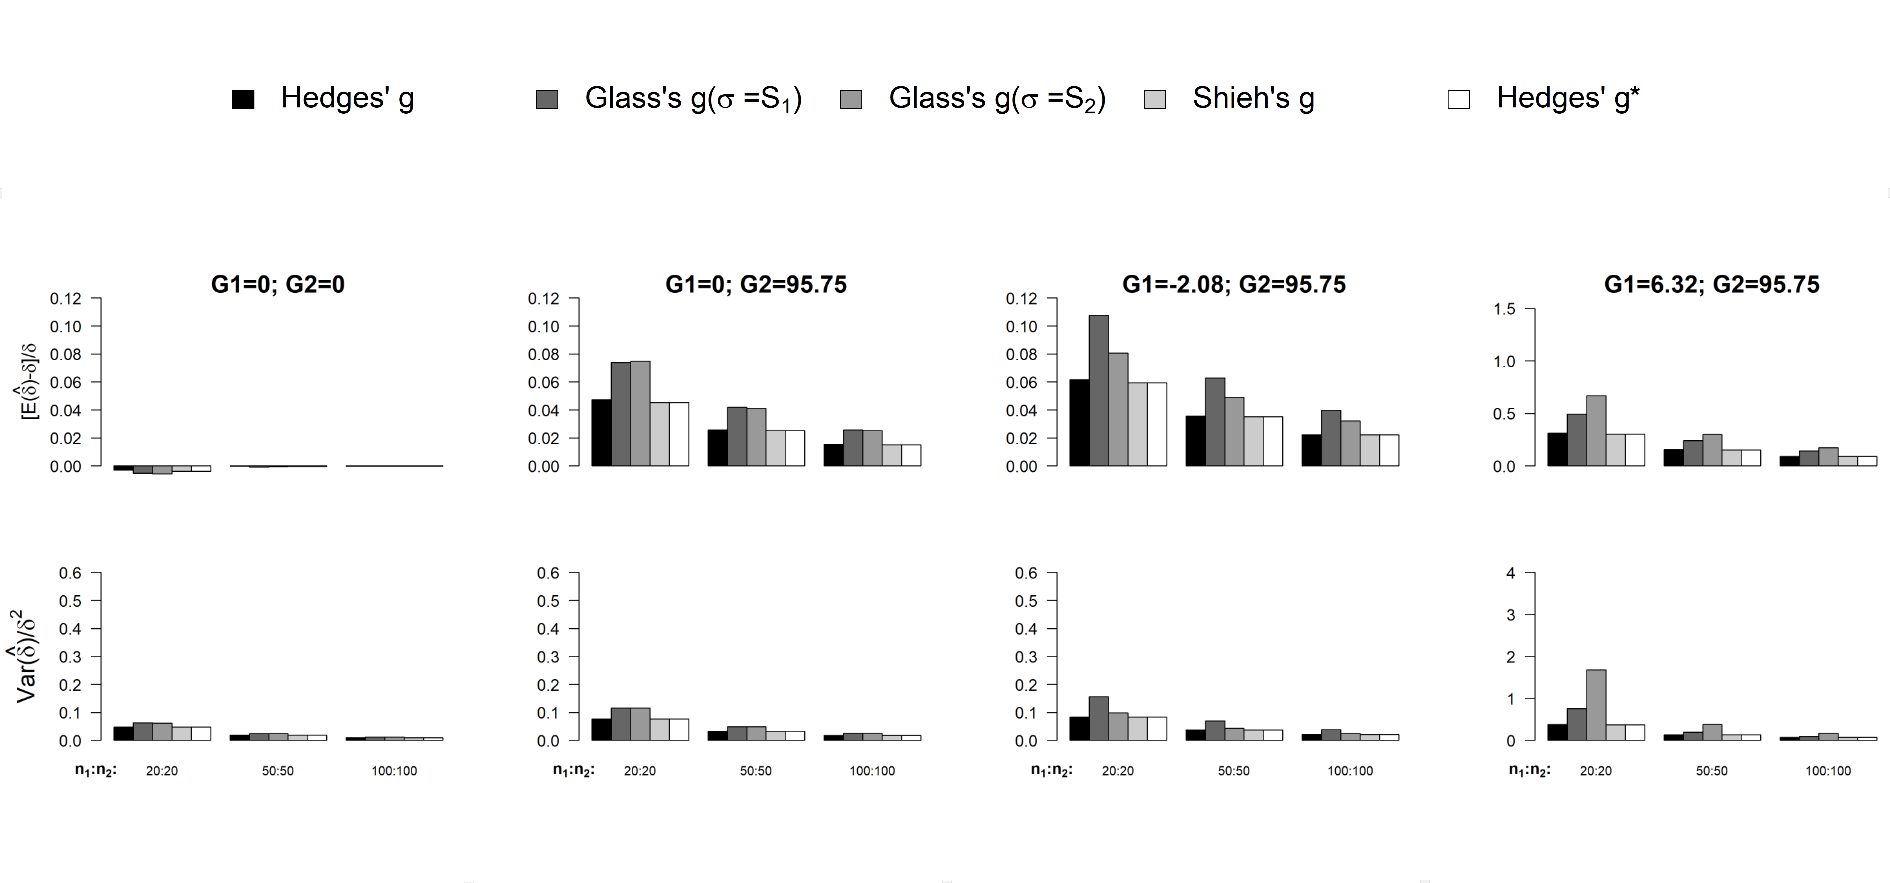
\includegraphics[width=1\linewidth]{C:/Users/mdelacre/Documents/Github projects/Effect-sizes/Scripts outputs/Quality of ES measures/Graphs/Unbiased estimators/Combined Figures_relative quality/Hom_bal} 

}

\caption{Bias and efficiency of estimators of standardized mean difference, when variances and sample sizes are equal across groups (condition a)}\label{fig:idHombal}
\end{figure}
\end{landscape}
\newpage
\begin{landscape}

\begin{figure}

{\centering 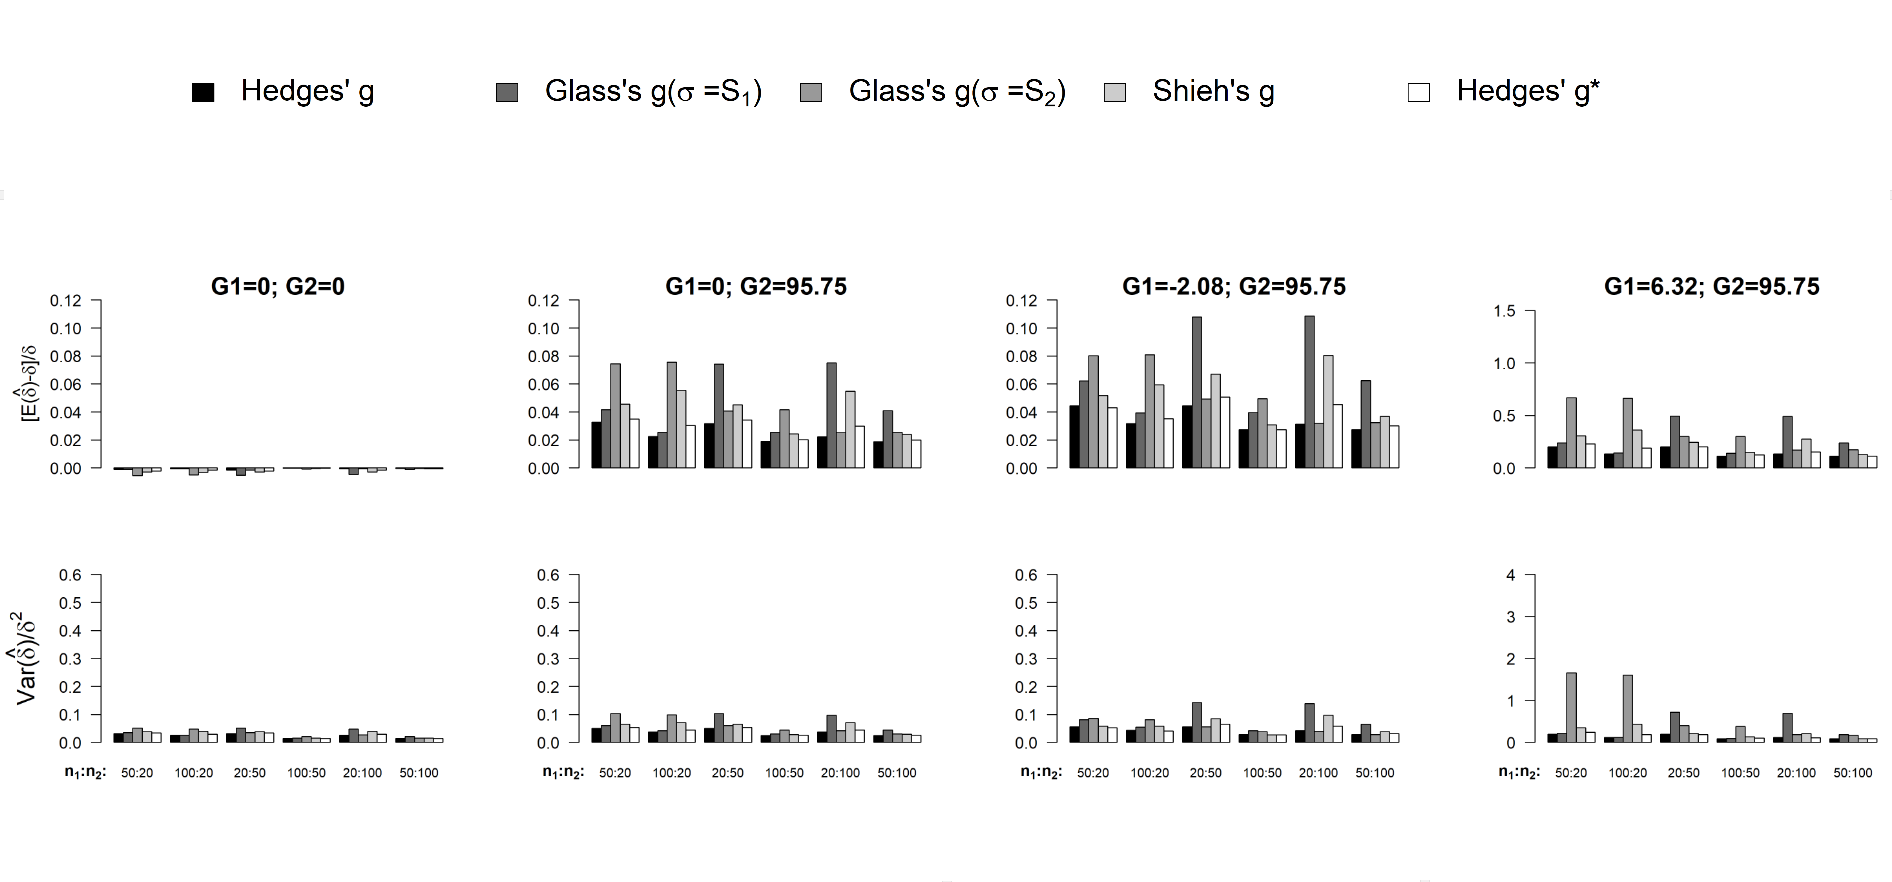
\includegraphics[width=1\linewidth]{C:/Users/mdelacre/Documents/Github projects/Effect-sizes/Scripts outputs/Quality of ES measures/Graphs/Unbiased estimators/Combined Figures_relative quality/Hom_unbal} 

}

\caption{Bias and efficiency of estimators of standardized mean difference, when variances are equal across groups and sample sizes are unequal (condition b)}\label{fig:idHomunbal}
\end{figure}

\end{landscape}

Figure \ref{fig:idHombal} illustrates scenarios where both population variances and sample sizes are equal across groups (condition a). One can first notice that all estimators are consistent, as their bias and variance decrease when the total sample size increases. For any departure from the normality assumption, both bias and variance of Hedges' \(g\), Shieh's \(g\) and Hedges' \(g^*\) are similar\footnote{While the bias and variance of Cohen's $d$, Cohen's $d^*$ and Shieh's $d$ are identical, the bias and variance of Hedges' $g$ are marginally different from the bias and variance of Hedges' $g^*$ and Shieh's $g$ (these last two having identical bias and variance). Indeed, because of the sampling error, differences remain between sample variances, even when population variances are equal between groups. Since the Hedges' correction applied to Cohen's $d$ does not contain the sample variances (unlike the correction applied on both other estimators), the bias and variance of Hedges' $g$ are slighly different from the bias and variance of Hedges' $g^*$ and Shieh's $g$.} and smaller than the bias and variance of Glass' \(g\) estimates using either \(S_1\) or \(S_2\) as a standardizer. Moreover, when samples are extracted from skewed distributions, Glass' \(g\) will show different bias and variance as a function of the chosen standardizer (\(S_1\) or \(S_2\)), even if both \(S_1\) and \(S_2\) are estimates of the same population variance, based on the same sample size. This is due to non-null correlations of opposite sign between the mean difference (\(\bar{X_1}-\bar{X_2}\)) and respectively \(S_1\) and \(S_2\). In Supplemental Material 3, we detailed in which situation a non-null correlation occurs between the sample mean difference (\(\bar{X_1}-\bar{X_2}\)) and the standardizer of compared estimators as well as the way this correlation impacts the bias and variance of estimators.

Figure \ref{fig:idHomunbal} illustrates scenarios where population variances are equal across groups, but sample sizes are unequal (condition b). For any departures from the normality assumptions, Hedges' \(g\) shows the smallest bias and variance. Hedges' \(g\) and Hedges' \(g^*\) are consistent estimators (i.e.~the larger the sample sizes, the lower the bias and the variance), unlike Shieh's \(g\) and Glass' \(g\). The bias of Glass' \(g\) does not depend either on the size of the experimental group or on the total sample size. The only way to decrease the bias of Glass' \(g\) is therefore to add subjects in the control group. On the other hand, the variance of Glass' \(g\) depends on both sample sizes, but not in an equivalent way : in order to reduce the variance, it is much more efficient to add subjects in the control group and when the relative size of the experimental group decreases so does the variance, even when the total sample size is decreased. Regarding Shieh's \(g\), for a given sample size ratio, the bias and variance will decrease when sample sizes increase. However, there is a large effect of the sample sizes ratio such that when the sample sizes ratio moves away from 1 by adding subjects, bias and variance might increase.\footnote{Regarding variance, in Supplemental Material 1, we mentioned that when the population effect size is zero, the larger the total sample size, the lower the variance, whether the sample sizes ratio is constant or not. We also mentioned that this is no longer true when the population effect size is not zero. In our simulations the effect size is never zero. The effect size effect is partially visible in Figure \ref{fig:idHomunbal} because we do not entirely remove the effect size effect when we divide the variance by $\delta^2$. This is due to the fact that one term, in the equation of the variance computation, does not depend on the effect size.} On the other hand, when the sample sizes ratio moves closer to 1 by adding subjects, the bias will decrease.

When samples are extracted from skewed distributions and have unequal sizes (the two last columns in Figure \ref{fig:idHomunbal}), for a constant total sample size, Glass' \(g\), Shieh's \(g\) and Hedges' \(g^*\) will show different bias and variance depending on which group is the largest one (e.g.~when distributions are right-skewed, the bias and variance of all these estimators when \(n_1\) and \(n_2\) are respectively 50 and 20 are not the same as their bias and variance when \(n_1\) and \(n_2\) are respectively 20 and 50). This is due to a non-null correlation of opposite sign between the mean difference (\(\bar{X_1}-\bar{X_2}\)) and their respective standardizers depending on which group is the largest one, as detailed in Supplemental Material 3. One observes that under these configurations, the bias and variance of Glass' \(g\) are sometimes a bit smaller and sometimes much larger than the bias and variance of Shieh's \(g\) and Cohen's \(d^*\).\footnote{Supplemental Material 3 shows that when $\mu_1-\mu_2 >0$ (like in our simulations), all other parameters being equal, an estimator is always less biased and variable when choosing a standardizer that is positively correlated with $\bar{X_1}-\bar{X_2}$. Supplemental Material 3 also shows that the smaller $n_c$, the larger the magnitude of correlation between $S_c$ and $\bar{X_1}-\bar{X_2}$. When $cor(S_c,\bar{X_1}-\bar{X_2})$ is positive, the positive effect of increasing the magnitude of the correlation is counterbalanced by the negative effect of reducing $n_c$. On the other hand, when $cor(S_c,\bar{X_1}-\bar{X_2})$ is negative, the negative effect of increasing the magnitude of the correlation is amplified by the negative effect of decreasing $n_c$. This explains why the difference between Glass' $g$ and other estimators is larger when Glass' $g$ is the least efficient estimator.}

\emph{When variances are unequal across groups}

Figures \ref{fig:idHetbal1} to \ref{fig:idHetunbal4} represent configurations where the equality of variances assumption is not met. According to our expectations, one observes that the bias of all estimators is approximately zero as long as the normality assumption is met (first column in all Figures), and the further from the normality assumption (i.e.~when moving from left to right in Figures), the larger the bias.\footnote{When looking at the relative bias for all estimators, the maximum departure from zero is 0.0173 when sample sizes are equal across groups, and 0.0274 when both sample sizes and variances differ across groups.}

We observe that when variances are unequal across populations, Glass' \(g\) sometimes performs better, but also sometimes performs much worse than Shieh's \(g\) and Hedges' \(g^*\), both in terms of bias and variance. The performance of Glass' \(g\) highly depends on parameters that we cannot control (i.e.~a triple interaction between the \(n\)-ratio, the \(SD\)-ratio and the correlation between the standardizer and the mean difference) and for this reason, we do not recommend using it. When the sample sizes ratio is close to 1, Shieh's \(g\) and Hedges' \(g^*\) are both appropriate but the further the sample sizes ratio is from 1, the larger the bias of Shieh's \(g\) such that, in the end, the measure that we believe performs best across scenarios is Hedges' \(g^*\).

\begin{landscape}
\newpage

\begin{figure}

{\centering 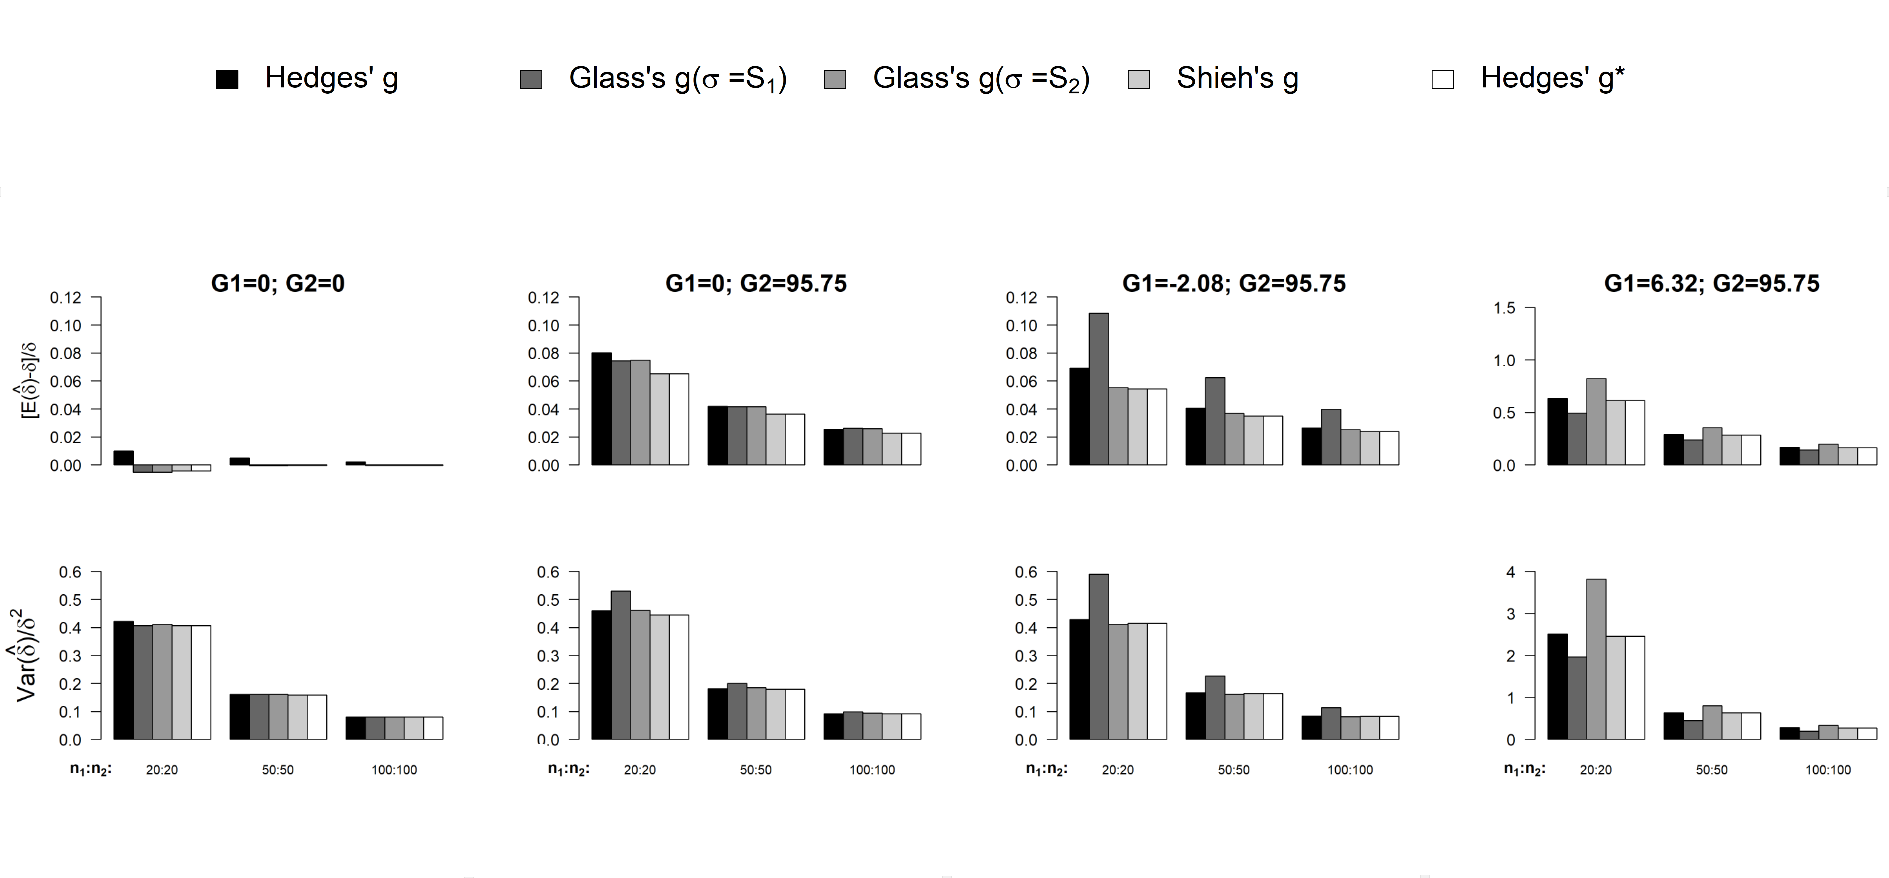
\includegraphics[width=1\linewidth]{C:/Users/mdelacre/Documents/Github projects/Effect-sizes/Scripts outputs/Quality of ES measures/Graphs/Unbiased estimators/Combined Figures_relative quality/Het_bal_N} 

}

\caption{Bias and efficiency of estimators of standardized mean difference, when variances are unequal across groups and sample sizes are equal (condition c), as a function of sample sizes}\label{fig:idHetbal1}
\end{figure}

\end{landscape}
\newpage
\begin{landscape}

\begin{figure}

{\centering 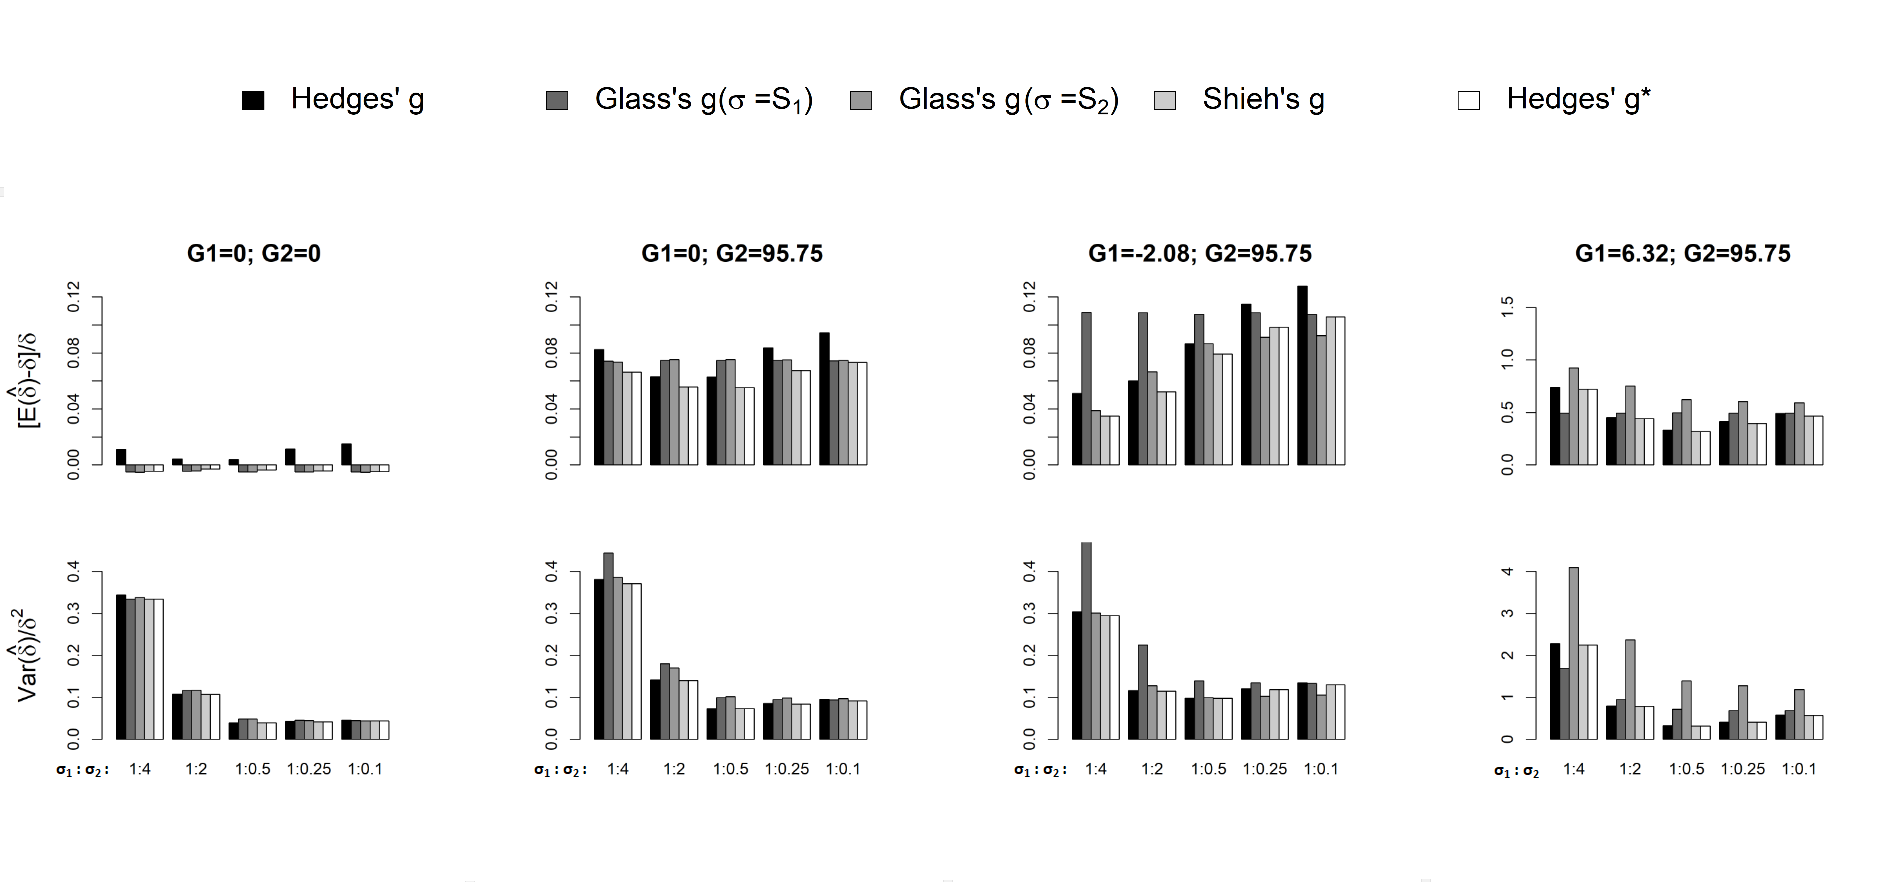
\includegraphics[width=1\linewidth]{C:/Users/mdelacre/Documents/Github projects/Effect-sizes/Scripts outputs/Quality of ES measures/Graphs/Unbiased estimators/Combined Figures_relative quality/Het_bal_sd} 

}

\caption{Bias and efficiency of estimators of standardized mean difference, when variances are unequal across groups and sample sizes are equal (condition c) as a function of the $SD$-ratio (when $n_1=n_2=20$)}\label{fig:idHetbal2}
\end{figure}

\end{landscape}
\newpage

Figures \ref{fig:idHetbal1} and \ref{fig:idHetbal2} are dedicated to scenarios where population variances are unequal between groups and sample sizes are equal (condition c). In Figure \ref{fig:idHetbal1}, scenarios are subdivided as a function of the sample sizes and one can notice that all estimators are consistent, as their bias and variance decrease when the total sample size increases. In Figure \ref{fig:idHetbal2}, scenarios are subdivided as a function of the \(SD\)-ratio. Because the comparison pattern remains very similar for all sample sizes, we present only scenarios when sample sizes equal 20. One should first notice that for all estimators in Figure \ref{fig:idHetbal2}, the relative variance seems to be much larger when \(S_2>S_1\).\footnote{The difference between the variance of estimators when the second group is 10 times larger than the first group was so large that we decided to not present it, for the sake of readability of the Figures.} This information should not be taken into account because it is only an artefact of our simulation conditions combined with the way we computed the relative variance.\footnote{We previously mentioned that when dividing the variance by $\delta^2$, we do not entirely remove the effect size effect. Actually, we introduce $\delta^2$ in the denominator of the first term, in the equation of the variance computation. Because we performed our simulations in order that $\sigma_1$ always equals 1, the smaller $S_2$, the larger the population effect size and therefore, the smaller the relative variance.}

When samples are extracted from skewed distributions, the bias and variance of Glass' \(g\) are sometimes smaller and sometimes larger than the bias of Shieh's \(g\) and Hedges' \(g^*\). This is mainly due to the fact that when two samples of same sizes are extracted from two skewed distributions with unequal variances (the two last columns in Figure \ref{fig:idHetbal2}), there will be non-null correlations of opposite sign between the mean difference (\(\bar{X_1}-\bar{X_2}\)) and the standardizer of \emph{all} estimators, depending on which population variance is larger.\footnote{When population variances are unequal, a non-null correlation occurs between standardizer estimates and $\bar{X_1}-\bar{X_2}$. For standardizers computed based on both $S_1$ and $S_2$, the sign of the correlation between the standardizer and the mean difference will be the same as the sign of the correlation between the mean difference and the estimate of the larger population variance. For interested readers, this is detailed in Supplemental Material 3.}

Figures \ref{fig:idHetunbal1} to \ref{fig:idHetunbal4} are dedicated to scenarios where both sample sizes and population variances differ across groups. Due to a high number of combinations between the sample sizes ratio and the \(SD\)-ratio in our simulations, we decided to present only some conditions. Because equations in Table 3 revealed an interaction effect between the sample sizes ratio and the \(SD\)-ratio on the bias and variance of Hedges' \(g^*\) and Shieh's \(g\) (see Supplemental Material 1), we chose to present all configurations where the larger \(SD\) is 10 times larger than the smaller \(SD\) (Figures \ref{fig:idHetunbal1} and \ref{fig:idHetunbal2}), and configurations where the larger \(SD\) is twice larger than the smaller \(SD\) (Figures \ref{fig:idHetunbal3} and \ref{fig:idHetunbal4}), in order to compare the effect of the sample sizes ratio on the bias and variance of all estimators when the \(SD\)-ratio is large (\(\frac{\sigma_2}{\sigma_1}=10 \; \mathrm{or} \; .1\) ) or medium (\(\frac{\sigma_2}{\sigma_1}=2 \; \mathrm{or} \; .5\)).

\begin{landscape}
\newpage

\begin{figure}

{\centering 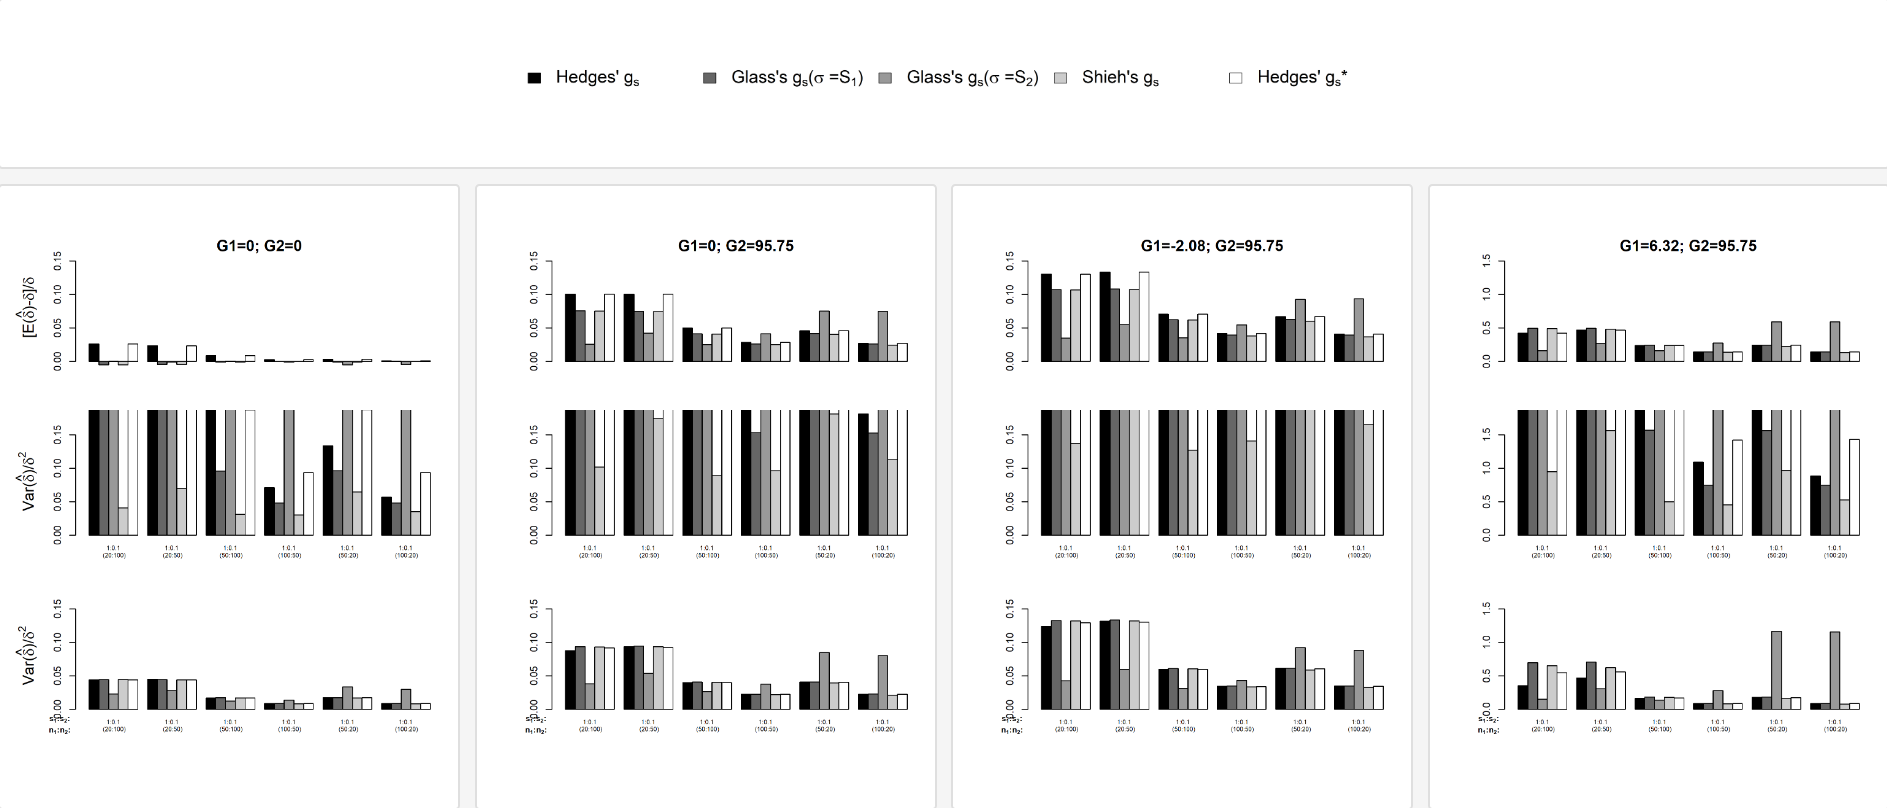
\includegraphics[width=1\linewidth]{C:/Users/mdelacre/Documents/Github projects/Effect-sizes/Scripts outputs/Quality of ES measures/Graphs/Unbiased estimators/Combined Figures_relative quality/Het_firstlarger_SDR10} 

}

\caption{Bias and efficiency of estimators of standardized mean difference, when variances and sample sizes are unequal across groups (condition d), and $\sigma_1$ is 10 times larger than $\sigma_2$}\label{fig:idHetunbal1}
\end{figure}

\end{landscape}
\newpage
\begin{landscape}

\begin{figure}

{\centering 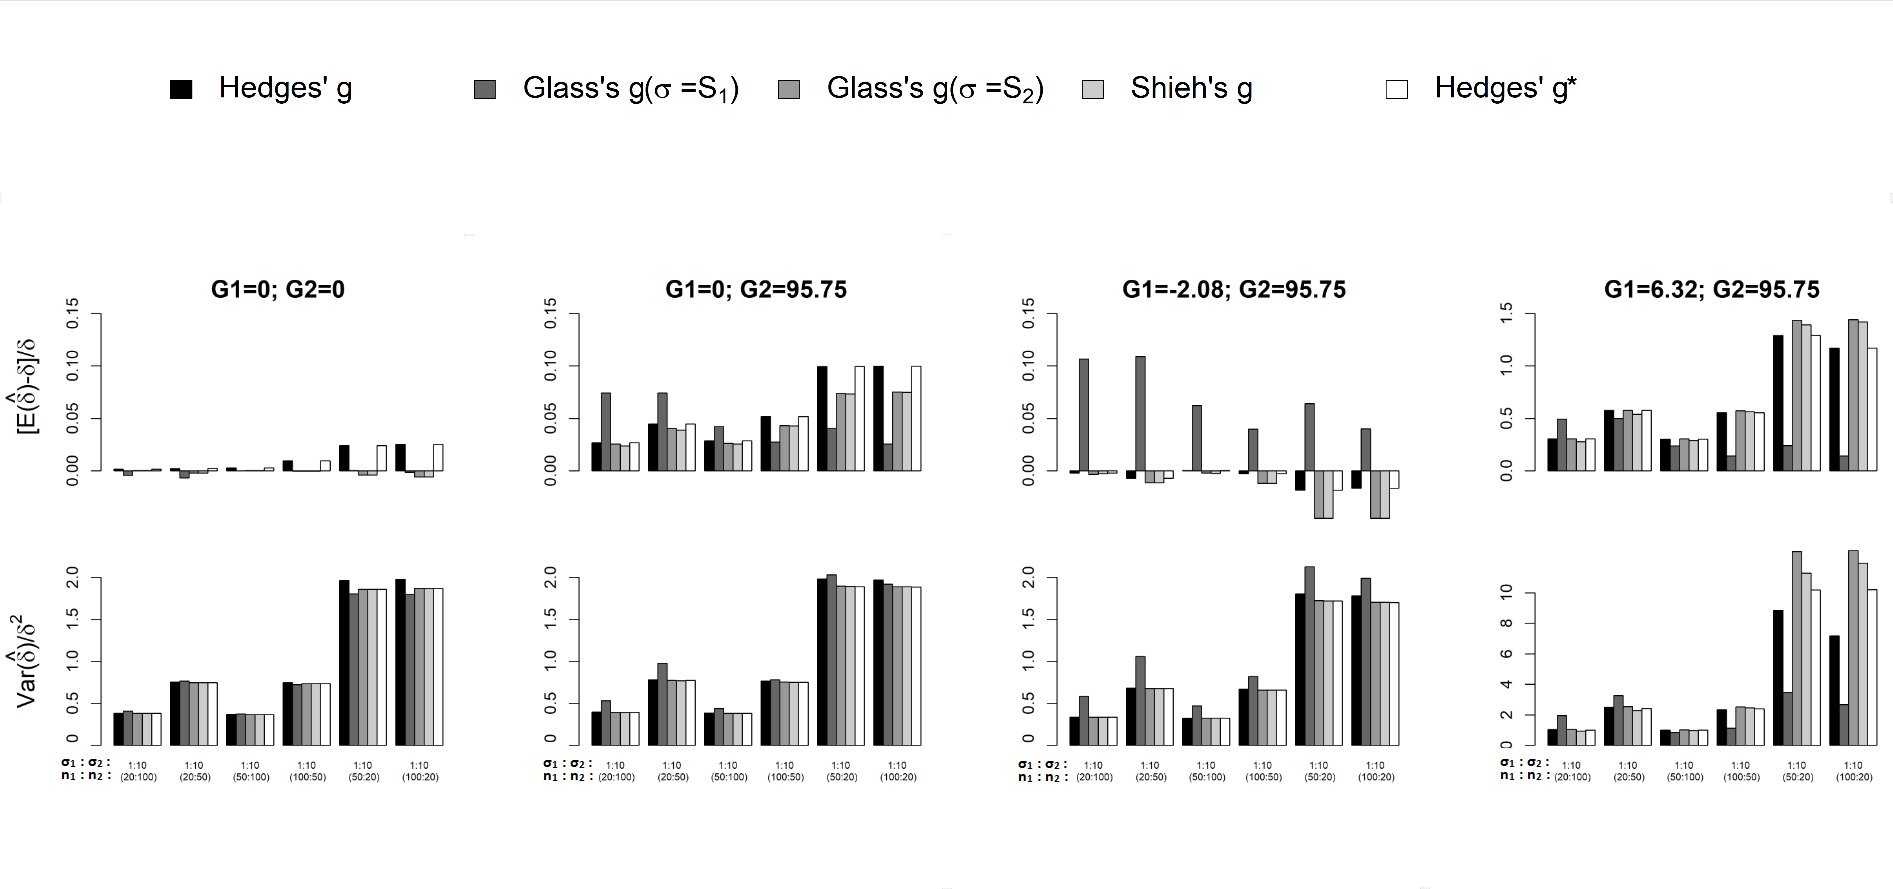
\includegraphics[width=1\linewidth]{C:/Users/mdelacre/Documents/Github projects/Effect-sizes/Scripts outputs/Quality of ES measures/Graphs/Unbiased estimators/Combined Figures_relative quality/Het_firstsmaller_SDR10} 

}

\caption{Bias and efficiency of estimators of standardized mean difference, when variances and sample sizes are unequal across groups (condition d), and $\sigma_2$ is 10 times larger than $\sigma_1$}\label{fig:idHetunbal2}
\end{figure}

\end{landscape}
\newpage
\begin{landscape}

\begin{figure}

{\centering 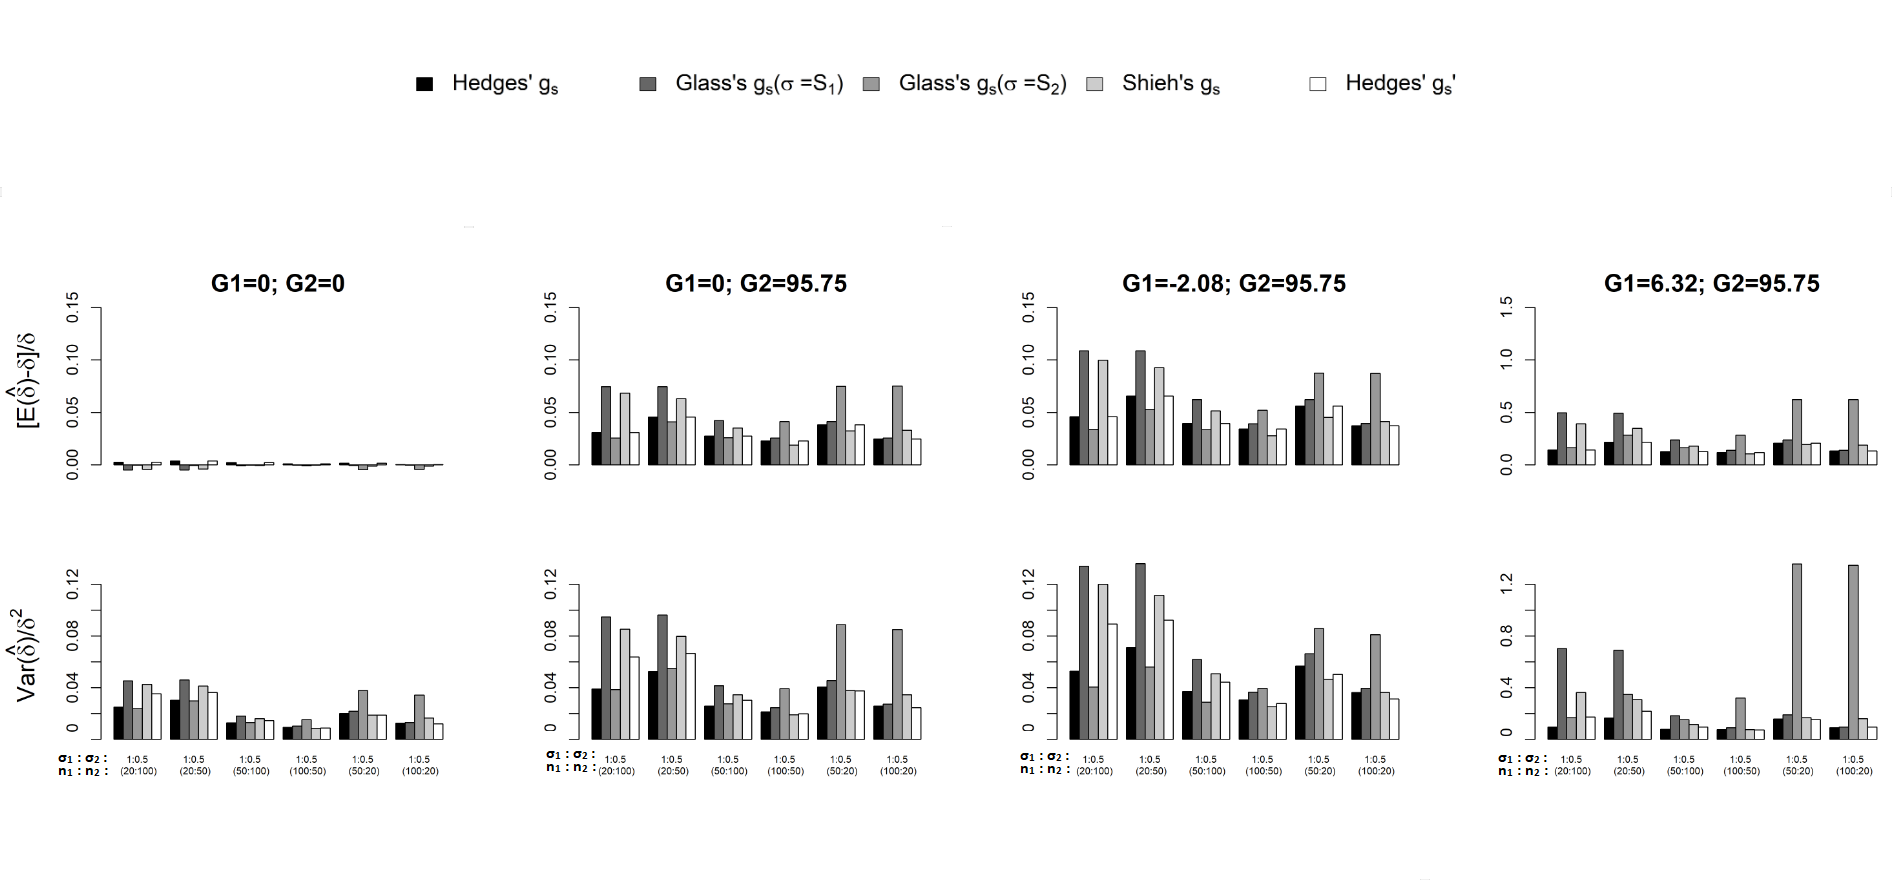
\includegraphics[width=1\linewidth]{C:/Users/mdelacre/Documents/Github projects/Effect-sizes/Scripts outputs/Quality of ES measures/Graphs/Unbiased estimators/Combined Figures_relative quality/Het_firstlarger_SDR2} 

}

\caption{Bias and efficiency of estimators of standardized mean difference, when variances and sample sizes are unequal across groups (condition d), and $\sigma_1$ is twice larger than $\sigma_2$}\label{fig:idHetunbal3}
\end{figure}

\end{landscape}
\newpage
\begin{landscape}

\begin{figure}

{\centering 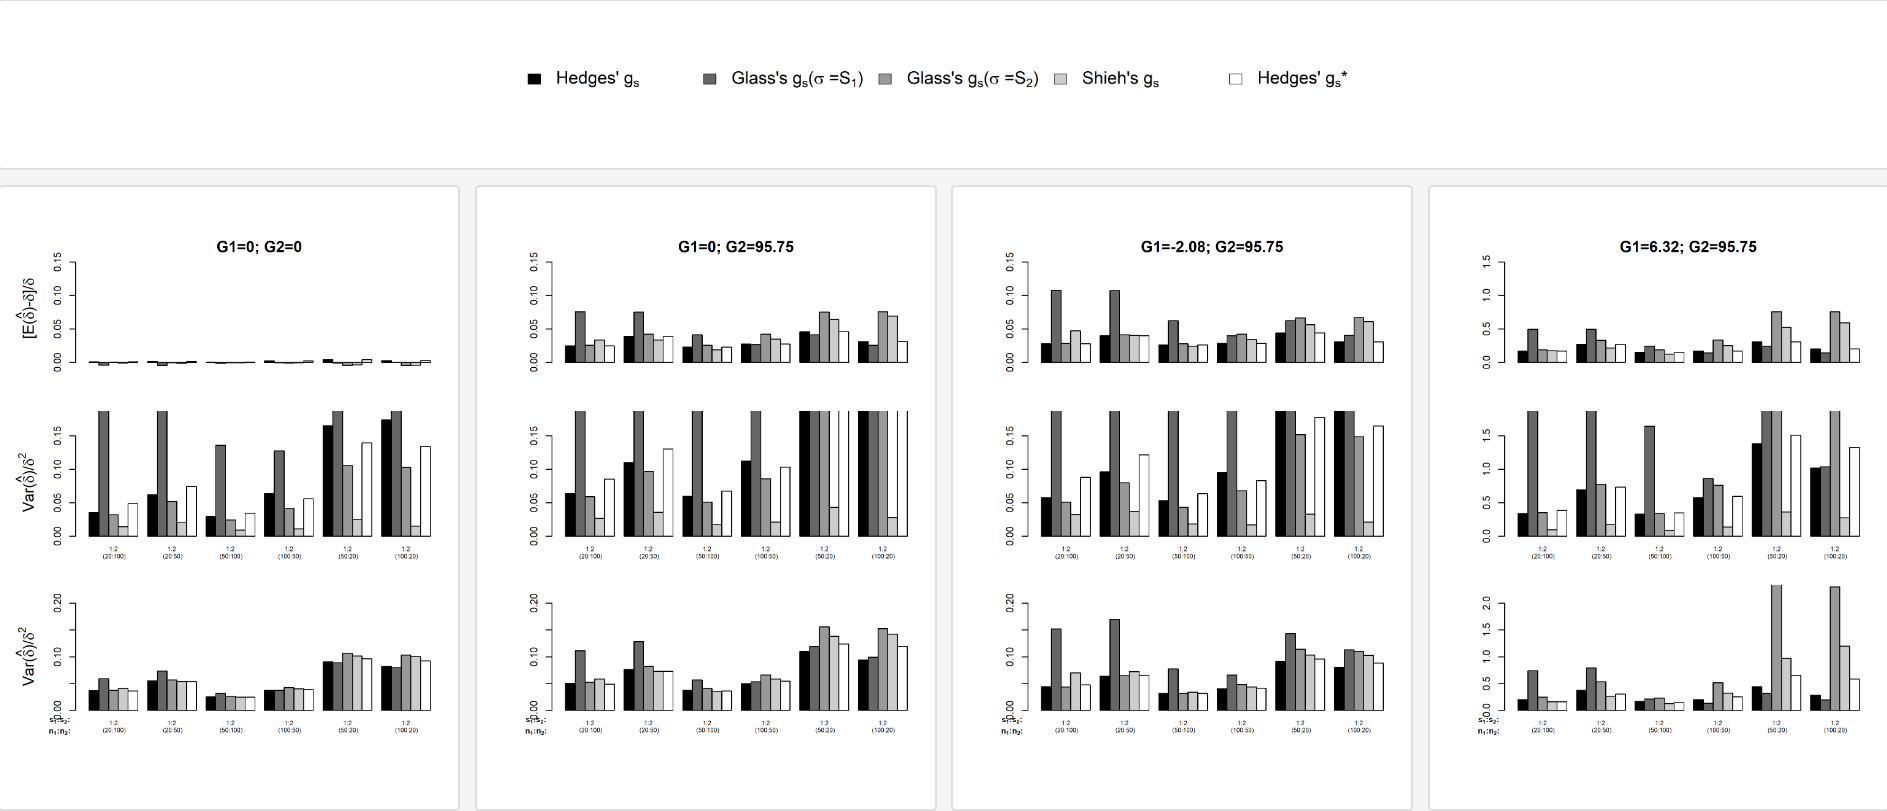
\includegraphics[width=1\linewidth]{C:/Users/mdelacre/Documents/Github projects/Effect-sizes/Scripts outputs/Quality of ES measures/Graphs/Unbiased estimators/Combined Figures_relative quality/Het_firstsmaller_SDR2} 

}

\caption{Bias and efficiency of estimators of standardized mean difference, when variances and sample sizes are unequal across groups (condition d), and $\sigma_2$ is twice larger than $\sigma_1$}\label{fig:idHetunbal4}
\end{figure}

\end{landscape}
\newpage

When distributions are symmetric, the bias of Glass' \(g\) only depends on the size of the control group and is therefore not impacted by either the sample sizes ratio or the total sample size. When comparing Figures \ref{fig:idHetunbal1} to \ref{fig:idHetunbal4}, one can also notice that the bias of Glass' \(g\) does not depend on the \(SD\)-ratio either. Unlike the bias of Glass' \(g\), its variance depends on both sample sizes, but not in an equivalent way. In most scenarios it is more efficient, in order to reduce the variance of Glass' \(g\), to add subjects in the control group. Regarding Hedges' \(g^*\) and Shieh's \(g\), their respective biases and variances depend on an interaction effect between the sample sizes ratio and the \(SD\)-ratio \(\left( \frac{n_2}{n_1} \times \frac{\sigma_2}{\sigma_1} \right)\) : the sample sizes ratio associated with the smallest bias and variance is not the same when the more variable group is 10 times more variable than the other group (Figures \ref{fig:idHetunbal1} and \ref{fig:idHetunbal2}) than when it is only twice more variable (Figures \ref{fig:idHetunbal3} and \ref{fig:idHetunbal4}). However, the respective biases and variances of Hedges' \(g^*\) and Shieh's \(g\) are always smaller when there is a positive pairing between sample sizes and variances. When samples are extracted from skewed distributions, the bias and variance of Glass' \(g\) are sometimes smaller and sometimes larger than the bias of Shieh's \(g\) and Hedges' \(g^*\), due to a combination of three factors : (1) which group is larger, (2) which group has the smallest standard deviation and (3) what is the correlation between the standardizer and the mean difference.

\hypertarget{recommendations-erceg-hurn_modern_2008}{%
\subsection{\texorpdfstring{Recommendations \color{white} Erceg-Hurn and Mirosevich (2008)\}}{Recommendations  Erceg-Hurn and Mirosevich (2008)\}}}\label{recommendations-erceg-hurn_modern_2008}}

\color{black}We recommend using Hedges' \(g^*\) in order to assess the magnitude of the effect when comparing two independent means, because a) it does not rely on the equality of population variances assumption \textbackslash footnote\{The assumption of equal variances across populations is rarely realistic in practice (Cain et al., 2017; Delacre et al., 2017; Delacre et al.~, 2019; Erceg-Hurn \(\&\) Mirosevich, 2008; Glass et al., 1972; Grissom, 2000; Micceri, 1989; Yuan et al., 2004) (unlike Hedges' \(g\)), b) it is always consistent (unlike Shieh's \(g\)), c) it is easy to interpret (Hedges' \(g^*\) can be interpreted in the same way as Hedges' \(g\)) and d) it remains constant for any sample sizes ratio, even when population variances are unequal across groups, as shown in the Shiny App at \url{https://effectsize.shinyapps.io/ShiehvsCohen/}.

Effect size estimates such as Hedges' \(g^*\) should always be reported with a confidence interval. To help researchers compute Hedges' \(g^*\) and its confidence interval we created the R package \emph{deffectsize} (see \url{https://github.com/mdelacre/deffectsize}). The \emph{datacohen\_CI} function was built in order to compute point estimators and confidence intervals based on raw data and the \emph{cohen\_CI} function was built in order to compute point estimators and confidence intervals based on descriptive statistics (sample means, sample variances and sample sizes). By default, unbiased Hedges' \(g^*\) is computed but it is also possible to compute biased estimators (e.g.~Cohen's \(d^*\)) and/or to use a pooled error term as standardizer by assuming that the equality of population variances is met (e.g.~Hedges' \(g\) or Cohen's \(d\), depending on whether we choose to compute unbiased or biased estimator). Other functions (\emph{datashieh\_CI}, \emph{shieh\_CI}, \emph{dataglass\_CI} and \emph{glass\_CI}) are available in order to compute Shieh's \(g\) (or Shieh's \(d\)) and Glass' \(g\) (or Glass' \(d\)) as well as their respective confidence intervals, even though we do not recommend to use these effect sizes by default. Researchers who do not use R can use a Shiny app to compute point estimators and confidence intervals based on descriptive statistics : \url{https://effectsize.shinyapps.io/deffsize/}.

\hypertarget{references}{%
\section{References}\label{references}}

\begingroup

\interlinepenalty = 10000

\hypertarget{refs}{}
\begin{CSLReferences}{1}{0}
\leavevmode\vadjust pre{\hypertarget{ref-algina_confidence_2006}{}}%
Algina, J., Keselman, H. J., \& Penfield, R. D. (2006). Confidence intervals for an effect size when variances are not equal. \emph{Journal of Modern Applied Statistical Methods}, \emph{5}(1), 2--13. \url{https://doi.org/10.22237/jmasm/1146456060}

\leavevmode\vadjust pre{\hypertarget{ref-altman_why_2005}{}}%
Altman, D. G. (2005). Why we need confidence intervals. \emph{World {J}ournal of {S}urgery}, \emph{29}(5), 554--556. \url{https://doi.org/10.1007/s00268-005-7911-0}

\leavevmode\vadjust pre{\hypertarget{ref-association_publication_2010}{}}%
American Psychological Association. (2010). \emph{Publication manual of the american psychological association {[}{APA}{]}} (6\(^{th}\) ed.). Washington, {DC}: American Psychological Association.

\leavevmode\vadjust pre{\hypertarget{ref-andersen_but_2007}{}}%
Andersen, M. B., McCullagh, P., \& Wilson, G. J. (2007). But what do the numbers really tell us?: Arbitrary metrics and effect size reporting in sport psychology research. \emph{Journal of {S}port and {E}xercise {P}sychology}, \emph{29}(5), 664--672. \url{https://doi.org/10.1123/jsep.29.5.664}

\leavevmode\vadjust pre{\hypertarget{ref-cain_univariate_2017}{}}%
Cain, M. K., Zhang, Z., \& Yuan, K.-H. (2017). Univariate and multivariate skewness and kurtosis for measuring nonnormality: Prevalence, influence and estimation. \emph{Behavior {R}esearch {M}ethods}, \emph{49}(5), 1716--1735. \url{https://doi.org/10.3758/s13428-016-0814-1}

\leavevmode\vadjust pre{\hypertarget{ref-coe_its_2002}{}}%
Coe, R. (2002). It's the effect size, stupid: What effect size is and why it is important. Paper presented at Annual Conference of the {B}ritish {E}ducational {R}esearch {A}ssociation, University of Exeter, Exeter, {U}nited-{K}ingdom.

\leavevmode\vadjust pre{\hypertarget{ref-cohen_statistical_1965}{}}%
Cohen, J. (1965). Some statistical issues in psychological research. In B. B. Wolmann (Ed.), \emph{Handbook of clinical psychology} (pp. 95--121). New York, NY: McGraw-Hill.

\leavevmode\vadjust pre{\hypertarget{ref-cumming_cohens_2013}{}}%
Cumming, G. (2013). Cohen's \emph{d} needs to be readily interpretable: Comment on shieh (2013). \emph{Behavior Research Methods}, \emph{45}(4), 968--971. \url{https://doi.org/10.3758/s13428-013-0392-4}

\leavevmode\vadjust pre{\hypertarget{ref-delacre_why_2017}{}}%
Delacre, M., Lakens, D., \& Leys, C. (2017). Why psychologists should by default use welch's \emph{t}-test instead of student's \emph{t}-test. \emph{International Review of Social Psychology}, \emph{30}(1), 92--101. \url{https://doi.org/10.5334/irsp.82}

\leavevmode\vadjust pre{\hypertarget{ref-duran_standards_2006}{}}%
Duran, R. P., Eisenhart, M. A., Erickson, F. D., Grant, C. A., Green, J. L., Hedges, L. V., \& Schneider, B. L. (2006). Standards for reporting on empirical social science research in {AERA} publications: {A}merican {E}ducational {R}esearch {A}ssociation. \emph{Educational Researcher}, \emph{35}(6), 33--40.

\leavevmode\vadjust pre{\hypertarget{ref-ellis_essential_2010}{}}%
Ellis, P. D. (2010). \emph{The essential guide to effect sizes: Statistical power, meta-analysis, and the interpretation of research results}. Cambridge, United-Kingdom: Cambridge University Press.

\leavevmode\vadjust pre{\hypertarget{ref-erceg-hurn_modern_2008}{}}%
Erceg-Hurn, D. M., \& Mirosevich, V. M. (2008). Modern robust statistical methods: An easy way to maximize the accuracy and power of your research. \emph{American Psychologist}, \emph{63}(7), 591--601. \url{https://doi.org/10.1037/0003-066X.63.7.591}

\leavevmode\vadjust pre{\hypertarget{ref-glass_meta-analysis_1981}{}}%
Glass, G. V., McGaw, B., \& Smith, M. L. (1981). \emph{Meta-analysis in social research}. Beverly Hills, {CA}: Sage.

\leavevmode\vadjust pre{\hypertarget{ref-goulet-pelletier_review_2018}{}}%
Goulet-Pelletier, J.-C., \& Cousineau, D. (2018). A review of effect sizes and their confidence intervals, part i: The cohen's \emph{d} family. \emph{The Quantitative Methods for Psychology}, \emph{14}(4), 242--265. \url{https://doi.org/10.20982/tqmp.14.4.p242}

\leavevmode\vadjust pre{\hypertarget{ref-grissom_heterogeneity_2000}{}}%
Grissom, R. J. (2000). Heterogeneity of variance in clinical data. \emph{Journal of Consulting and Clinical Psychology}, \emph{68}(1), 155--165. \url{https://doi.org/10.1037/0022-006X.68.1.155}

\leavevmode\vadjust pre{\hypertarget{ref-grissom_review_2001}{}}%
Grissom, R. J., \& Kim, J. J. (2001). Review of assumptions and problems in the appropriate conceptualization of effect size. \emph{Psychological Methods}, \emph{6}(2), 135--146. \url{https://doi.org/10.1037/1082-989X.6.2.135}

\leavevmode\vadjust pre{\hypertarget{ref-grissom_effect_2005}{}}%
Grissom, R. J., \& Kim, J. J. (2005). \emph{Effect sizes for research: A broad practical approach}. Mahwah, NJ: Lawrence Erlbaum Associates.

\leavevmode\vadjust pre{\hypertarget{ref-hedges_statistical_1985}{}}%
Hedges, L. V., \& Olkin, I. (1985). \emph{Statistical methods for meta-analysis}. Orlando, FL: Academic Press.

\leavevmode\vadjust pre{\hypertarget{ref-huynh_unified_1989}{}}%
Huynh, C.-L. (1989). A unified approach to the estimation of effect size in meta-analysis. Paper presented at the {A}nnual {M}eeting of the {A}merican {E}ducational {R}esearch {A}ssociation, San Francisco, CA.

\leavevmode\vadjust pre{\hypertarget{ref-kelley_effects_2005}{}}%
Kelley, K. (2005). The effects of nonnormal distributions on confidence intervals around the standardized mean difference: Bootstrap and parametric confidence intervals. \emph{Educational and Psychological Measurement}, \emph{65}(1), 51--69. \url{https://doi.org/10.1177/0013164404264850}

\leavevmode\vadjust pre{\hypertarget{ref-keselman_generally_2008}{}}%
Keselman, H. J., Algina, J., Lix, L. M., Wilcox, R. R., \& Deering, K. N. (2008). A generally robust approach for testing hypotheses and setting confidence intervals for effect sizes. \emph{Psychological Methods}, \emph{13}(2), 110--129. \url{https://doi.org/10.1037/1082-989X.13.2.110}

\leavevmode\vadjust pre{\hypertarget{ref-kulinskaya_confidence_2007}{}}%
Kulinskaya, E., \& Staudte, R. G. (2007). Confidence intervals for the standardized effect arising in the comparison of two normal populations. \emph{Statistics in Medicine}, \emph{26}(14), 2853--2871. \url{https://doi.org/10.1002/sim.2751}

\leavevmode\vadjust pre{\hypertarget{ref-lakens_calculating_2013}{}}%
Lakens, D. (2013). Calculating and reporting effect sizes to facilitate cumulative science: A practical primer for \emph{t}-tests and {ANOVAs}. \emph{Frontiers in Psychology}, \emph{4}(863), 1--12. \url{https://doi.org/10.3389/fpsyg.2013.00863}

\leavevmode\vadjust pre{\hypertarget{ref-peng_impact_2013}{}}%
Peng, C.-Y. J., Chen, L.-T., Chiang, H.-M., \& Chiang, Y.-C. (2013). The impact of {APA} and {AERA} guidelines on effect size reporting. \emph{Educational Psychology Review}, \emph{25}(2), 157--209. \url{https://doi.org/10.1007/s10648-013-9218-2}

\leavevmode\vadjust pre{\hypertarget{ref-prentice_when_1992}{}}%
Prentice, D. A., \& Miller, D. T. (1992). When small effects are impressive. \emph{Psychological Bulletin}, \emph{112}(1), 160--164. \url{https://doi.org/10.1037/0033-2909.112.1.160}

\leavevmode\vadjust pre{\hypertarget{ref-raviv_bias_2014}{}}%
Raviv, E. (2014, June 2). Bias vs. consistency. Retrieved July 12, 2021, from \url{https://eranraviv.com/bias-vs-consistency/}

\leavevmode\vadjust pre{\hypertarget{ref-shieh_confidence_2013}{}}%
Shieh, G. (2013). Confidence intervals and sample size calculations for the standardized mean difference effect size between two normal populations under heteroscedasticity. \emph{Behavior Research Methods}, \emph{45}(4), 955--967. \url{https://doi.org/10.3758/s13428-013-0320-7}

\leavevmode\vadjust pre{\hypertarget{ref-stout_assessing_1995}{}}%
Stout, D. E., \& Ruble, T. L. (1995). Assessing the practical significance of empirical results in accounting education research: The use of effect size information. \emph{Journal of Accounting Education}, \emph{13}(3), 281--298. \url{https://doi.org/10.1016/0748-5751(95)00010-J}

\leavevmode\vadjust pre{\hypertarget{ref-sullivan_using_2012}{}}%
Sullivan, G. M., \& Feinn, R. (2012). Using effect size---or why the \emph{p} value is not enough. \emph{Journal of Graduate Medical Education}, \emph{4}(3), 279--282. \url{https://doi.org/10.4300/JGME-D-12-00156.1}

\leavevmode\vadjust pre{\hypertarget{ref-welch_significance_1938}{}}%
Welch, B. L. (1938). The significance of the difference between two means when the population variances are unequal. \emph{Biometrika}, \emph{29}(3), 350--362. \url{https://doi.org/10.2307/2332010}

\leavevmode\vadjust pre{\hypertarget{ref-wilkinson_statistical_1999}{}}%
Wilkinson, L. (1999). Statistical methods in psychology journals: Guidelines and explanations. \emph{American Psychologist}, \emph{54}(8), 594--604. \url{https://doi.org/10.1037/0003-066X.54.8.594}

\end{CSLReferences}

\endgroup


\clearpage
\makeatletter
\efloat@restorefloats
\makeatother


\begin{appendix}
\section{}
\hypertarget{the-bias-of-cohens-bmd-is-twice-as-large-as-the-bias-of-shiehs-bmd-when-population-variances-and-sample-sizes-are-equal-across-groups-mathematical-demonstration.}{%
\subsection{\texorpdfstring{The bias of Cohen's \(\bm{d}\) is twice as
large as the bias of Shieh's \(\bm{d}\) when population variances and
sample sizes are equal across groups: mathematical
demonstration.}{The bias of Cohen's \textbackslash bm\{d\} is twice as large as the bias of Shieh's \textbackslash bm\{d\} when population variances and sample sizes are equal across groups: mathematical demonstration.}}\label{the-bias-of-cohens-bmd-is-twice-as-large-as-the-bias-of-shiehs-bmd-when-population-variances-and-sample-sizes-are-equal-across-groups-mathematical-demonstration.}}

As mentioned in Table 1, the bias of Cohen's \(d\) is defined as
\begin{equation} 
Bias_{Cohen's \; d}= \delta_{Cohen} \times \left( \frac{\sqrt{\frac{df_{Student}}{2}} \times \Gamma{\left(\frac{df_{Student}-1}{2}\right)}}{\Gamma{\left( \frac{df_{Student}}{2}\right)}} -1 \right)
\label{eq:Cohenbias}
\end{equation} with \begin{equation*} 
\delta_{Cohen}=\frac{\mu_1-\mu_2}{\sqrt{\frac{(n_1-1)\times \sigma^2_1+(n_2-1)\times\sigma^2_2}{n_1+n_2-2}}}
\label{eq:Cohendelta}
\end{equation*} and \begin{equation*} 
df_{Student}=n_1+n_2-2
\label{eq:Cohendf}
\end{equation*}

As mentioned in Table 2, the bias of Shieh's \(d\) is defined as
\begin{equation} 
Bias_{Shieh's \; d}=\delta_{Shieh} \times \left( \frac{\sqrt{\frac{df_{Welch}}{2}} \times \Gamma{\left(\frac{df_{Welch}-1}{2}\right)}}{\Gamma{\left( \frac{df_{Welch}}{2}\right)}} -1 \right)
\label{eq:Shiehbias}
\end{equation} with \begin{equation*} 
\delta_{Shieh}=\frac{\mu_1-\mu_2}{\sqrt{\frac{\sigma^2_1}{n_1/N}+\frac{\sigma^2_2}{n_2/N}}} \quad (N=n_1+n_2)
\label{eq:Shiehdelta}
\end{equation*} and \begin{equation*} 
df_{Welch}=\frac{\left(\frac{\sigma^2_1}{n_1}+\frac{\sigma^2_2}{n_2} \right)^2}{\frac{(\sigma^2_1/n_1)^2}{n_1-1}+\frac{(\sigma^2_2/n_2)^2}{n_2-1}}
\label{eq:Welchdf}
\end{equation*}

When \(n_1=n_2=n\) and \(\sigma_1=\sigma_2=\sigma\), \(\delta_{Cohen}\)
is twice larger than \(\delta_{Shieh}\), as shown below in equations
\ref{eq:Cohendeltavarbalanced} and \ref{eq:Shiehdeltavarbalanced}:
\begin{equation} 
\delta_{Cohen}=\frac{\mu_1-\mu_2}{\sqrt{\frac{2(n-1)\sigma^2}{2(n-1)}}}=\bm{\frac{\mu_1-\mu_2}{\sigma}}
\label{eq:Cohendeltavarbalanced}
\end{equation} \begin{equation} 
\delta_{Shieh}=\frac{\mu_1-\mu_2}{\sqrt{2\left( \frac{\sigma^2}{n/(2n)}\right)}}=\bm{\frac{\mu_1-\mu_2}{2\sigma}} 
\label{eq:Shiehdeltavarbalanced}
\end{equation}\\
Moreover, degrees of freedom associated with Student's \emph{t}-test and
Welch's \emph{t}-test are identical, as shown below in equations
\ref{eq:Studentdfvarbalanced} and \ref{eq:Welchdfvarbalanced}:
\begin{equation} 
df_{Student}=\bm{2(n-1)} 
\label{eq:Studentdfvarbalanced}
\end{equation} \begin{equation} 
df_{Welch}=\frac{\left[2(\sigma^2/n)\right]^2}{\frac{2(\sigma^2/n)^2}{n-1}}= \bm{2(n-1)} 
\label{eq:Welchdfvarbalanced}
\end{equation}

Equations \ref{eq:Cohenbias} and \ref{eq:Shiehbias} can therefore be
redefined as follows: \begin{equation} 
Bias_{Cohen's \; d}=\frac{\mu_1-\mu_2}{\sigma} \times \left( \frac{\sqrt{n-1} \times \Gamma{\left(\frac{2n-3}{2}\right)}}{\Gamma{\left( n-1\right)}} -1 \right)
\label{eq:Cohenbiasvarbalanced}
\end{equation} \begin{equation} 
Bias_{Shieh's \; d}=\frac{\mu_1-\mu_2}{\bf 2\sigma} \times \left( \frac{\sqrt{n-1} \times \Gamma{\left(\frac{2n-3}{2}\right)}}{\Gamma{\left( n-1\right)}} -1 \right)
\label{eq:Shiehbiasvarbalanced}
\end{equation}

We can therefore conclude that the bias of Cohen's \(d\) is twice larger
than the bias of Shieh's \(d\).

\newpage

\hypertarget{the-variance-of-cohens-bmd-is-four-times-larger-than-the-bias-of-shiehs-bmd-when-population-variances-and-sample-sizes-are-equal-across-groups-mathematical-demonstration.}{%
\subsection{\texorpdfstring{The variance of Cohen's \(\bm{d}\) is four
times larger than the bias of Shieh's \(\bm{d}\) when population
variances and sample sizes are equal across groups: mathematical
demonstration.}{The variance of Cohen's \textbackslash bm\{d\} is four times larger than the bias of Shieh's \textbackslash bm\{d\} when population variances and sample sizes are equal across groups: mathematical demonstration.}}\label{the-variance-of-cohens-bmd-is-four-times-larger-than-the-bias-of-shiehs-bmd-when-population-variances-and-sample-sizes-are-equal-across-groups-mathematical-demonstration.}}

The variance of Cohen's \(d\) is defined in Table 1 as \begin{equation}
Var_{Cohen's \; d}=\frac{N\times df_{Student}}{n_1n_2 \times (df_{Student}-2)} + \delta^2_{Cohen} \left[ \frac{df_{Student}}{df_{Student}-2} - \left( \frac{\sqrt{\frac{df_{Student}}{2}} \times \Gamma{\left(\frac{df_{Student}-1}{2}\right)}}{\Gamma{\left( \frac{df_{Student}}{2}\right)}} \right)^2\right]
\label{eq:Cohenvar}
\end{equation} and the variance of Shieh's \(d\) is defined in Table 2
as \begin{equation}
Var_{Shieh's \; d}=\frac{df_{Welch}}{(df_{Welch}-2)N}  + \delta^2_{Shieh} \left[ \frac{df_{Welch}}{df_{Welch}-2} - \left( \frac{\sqrt{\frac{df_{Welch}}{2}} \times \Gamma{\left(\frac{df_{Welch}-1}{2}\right)}}{\Gamma{\left( \frac{df_{Welch}}{2}\right)}} \right)^2 \right]
\label{eq:Shiehvar}
\end{equation}

We have previously shown in equations \ref{eq:Studentdfvarbalanced} and
\ref{eq:Welchdfvarbalanced} that degrees of freedom associated with
Student's \emph{t}-test and Welch's \emph{t}-test equal \(2(n-1)\), when
\(n_1=n_2=n\) and \(\sigma_1=\sigma_2=\sigma\). As a consequence, the
first term of the addition in equation \ref{eq:Cohenvar} is 4 times
larger than the first term of the addition in equation
\ref{eq:Shiehvar}:
\[\frac{N\times df_{Student}}{n_1n_2 \times (df_{Student}-2)}=\frac{2n\times 2(n-1)}{n^2 \times (2n-4)} =\bm{\frac{4(n-1)}{n(2n-4)}} \]
\[\frac{df_{Welch}}{(df_{Welch}-2)N} = \frac{2(n-1)}{2n(2n-4)}= \bm{\frac{n-1}{n(2n-4)}}\]
We have also previously shown in equations
\ref{eq:Cohendeltavarbalanced} and \ref{eq:Shiehdeltavarbalanced} that
\(\delta_{Cohen}\) is twice larger than \(\delta_{Shieh}\) when
\(n_1=n_2=n\) and \(\sigma_1=\sigma_2=\sigma\) and, therefore,
\(\delta^2_{Cohen}\) is four times larger than \(\delta^2_{Shieh}\). As
a consequence, the second term of the addition in equation
\ref{eq:Cohenvar} is also 4 times larger than the second term of the
addition in equation \ref{eq:Shiehvar}. Because both terms of the
addition in equation \ref{eq:Cohenvar} are four times larger than those
in equation \ref{eq:Shiehvar}, we can conclude that the variance of
Cohen's \(d\) is four times larger than the variance of Shieh's \(d\).
\end{appendix}

\end{document}
